\documentclass{article} % For LaTeX2e
\usepackage{iclr2027_conference,times}

\input{math_commands.tex}

\usepackage{hyperref}
\usepackage{url}
\usepackage{graphicx}
\usepackage{booktabs}
\usepackage{multirow}
\usepackage{amsmath,amssymb}
\usepackage{subcaption}
\usepackage{xcolor}

% Float packing: allow text and floats to share pages more aggressively than
% the LaTeX defaults, which otherwise leave large gaps in a figure-heavy paper.
\renewcommand{\topfraction}{0.92}
\renewcommand{\bottomfraction}{0.85}
\renewcommand{\textfraction}{0.07}
\renewcommand{\floatpagefraction}{0.8}
\setcounter{topnumber}{3}
\setcounter{bottomnumber}{2}
\setcounter{totalnumber}{4}

% Compact float spacing
\setlength{\textfloatsep}{12pt plus 2pt minus 4pt}
\setlength{\abovecaptionskip}{6pt}

% Internal revision commands
\newcommand{\todo}[1]{{\color{red}[TODO: #1]}}
\newcommand{\model}{DMF-Gen-3D}

\title{Scalable Generative Reconstruction of\\Three-Dimensional Fields on Point Clouds}

% Authors hidden for submission; \iclrfinalcopy reveals them.
\author{Nicolas Tricard, Linzheng Wang, Jason Chen, Sili Deng \\
Department of Mechanical Engineering\\
Massachusetts Institute of Technology\\
Cambridge, MA 02139, USA \\
\texttt{\{ntricard,wanglz,jachen25,silideng\}@mit.edu} \\
}

%\iclrfinalcopy % Uncomment for camera-ready version, but NOT for submission.
\begin{document}

\maketitle

\begin{abstract}
Reconstructing three-dimensional physical fields from sparse measurements is an ill-posed inverse problem for which generative models provide the natural formulation: they sample from the distribution over fields consistent with the data rather than regressing to its mean. Current methods do not survive the transition to three dimensions---voxel diffusion computes globally on dense grids and hits a measured memory wall, while latent methods compress fields through an autoencoder that bounds what can be recovered. We introduce \model{}, a conditional rectified-flow model that generates fields directly in ambient function space, on arbitrary point clouds, with no autoencoder and no voxelization. Each query point is conditioned through a compact global summary of the observations and a local, importance-weighted retrieval over sensor tokens; the training objective, an integral over the domain, is estimated on a random $\sim$2\% subset of points per step, decoupling training cost from resolution. A single model is amortized over sensor counts, layouts, noise levels, and observed-channel patterns. Its training memory is constant from $64^3$ to $1024^3$ output resolution, where voxel diffusion and the autoencoder hit measured walls at $320^3$ and $640^3$, and its inference is constant-memory with time linear in the number of evaluation points. The capability this buys is evaluated where no grid exists: \model{} infers volumetric predictive distributions from surface-only sensors on unstructured transonic-wing meshes---a measurement operator grid-based generative methods cannot represent without resampling---and under noisy, occluded, and channel-dropped sensing on wildfire simulation its worst-case error is below every baseline's best case. On a controlled periodic-grid turbulence benchmark, where voxel and patch methods operate on their native terrain, ten upstream-audited baselines bracket \model{}: no method leads every column, and \model{} trails the per-channel leader on observed channels by at most $0.04$ relative $L_2$ while sampling in $2$--$4$ network evaluations against their $32$--$1000$, with the strongest member-level dissipation-range spectral fidelity of the generative methods measured. Throughout, we characterize the predictive uncertainty rather than assume it---a density-invariant spread--distance profile with a hard floor---and repair it post hoc by conformal recalibration fitted on a disjoint tuning split.\todo{Verify recalibration claim once TEST-split fits land; soften to ``characterize'' if repair underdelivers.}
\end{abstract}

\section{Introduction}
\label{sec:intro}

Volumetric fields govern systems that experiments can only observe pointwise: velocimetry resolves planes of a turbulent flow while the surrounding volume goes unmeasured, and flight-test campaigns record surface pressure at taps while the off-body flow that determines performance is inaccessible. Recovering the full three-dimensional state is a long-standing inverse problem \citep{callaham2019robust,raissi2020hidden,vinuesa2023transformative}, and at realistic sensor densities it is severely ill-posed: many fields fit the data, and the missing information sits disproportionately at the small scales. Deterministic reconstruction networks \citep{fukami2021global,santos2023senseiver,dang2025flronet} return a conditional mean---the optimal point estimate and a systematically over-smoothed one, blurring precisely the fine structure whose recovery motivates reconstruction. That collapse is structural rather than a training-budget artifact: turbulent solution maps carry infinitesimally separated inputs to macroscopically different outputs, while trained networks are biased toward smooth, insensitive maps, so a squared-error objective is minimized by the mean of the conditional distribution and ensembles of such models inherit the same limit \citep{raonic2026gencfd}. Generative models resolve the mismatch by sampling fields consistent with the observations, retaining sharp realizations and quantifying what the measurements leave undetermined \citep{shu2023physics,li2024s3gm,zhuang2025spatially}.

This posterior-sampling program has largely been carried out in two dimensions \citep{shu2023physics,amoros2026guiding,li2024s3gm,huang2024diffusionpde,zhuang2025spatially}. In parallel, generative modeling has been lifted from fixed grids to function space, defining flows over functions that are consistent across discretizations \citep{kerrigan2024functional,lim2025score,pidstrigach2024infinite,shi2025stochastic}, with guided variants for inverse problems \citep{yao2025fundps,kerrigan2024dynamic}. These methods establish the right abstraction for scattered measurements, but their demonstrations remain at $64\times64$ to $128\times128$ on uniform grids with spectral backbones that presuppose them; scaling guided function-space sampling beyond two dimensions is stated as an open problem \citep{yao2025fundps}.

The transition to three dimensions has been attempted along two detours, each with a documented cost. The first is voxelization: dense 3D U-Nets and transformers compute globally on the full grid at every step, so activation memory grows with the cube of resolution, and published 3D generative models cap their domains at $192\times48\times48$ \citep{lienen2024zero}, train on $32^3$ crops with attention removed \citep{oommen2026turbulent}, factorize attention at $64^3$ \citep{li2023factformer}, or resort to patch decompositions \citep{holzschuh2026pd3}; it also forfeits the geometry, since unstructured meshes must first be resampled onto axis-aligned grids. The second is latent compression \citep{du2024confild,zhou2025text2pde,wang2026fundiff,li2025latent}, which makes 3D generation affordable but bounds reconstruction by the autoencoder, and that bound is not tight enough for turbulence: MSE-trained autoencoders retain roughly a quarter of the spectral power in the dissipation range \citep{rafiq2026spectrally,glaws2020deep}, and latent neural-field models report small-scale discrepancies on their own benchmarks \citep{du2024confild}. A model whose prior cannot represent the small scales cannot return them, whatever the observations. Meanwhile the architectures that do scale to realistic 3D discretizations \citep{luo2025transolver,alkin2024upt,alkin2025abupt,li2023gino} are uniformly deterministic, and generative modeling on meshes has been limited to a few thousand nodes \citep{lino2025dgn}.

A further gap separates published evaluations from deployed sensing. The dominant protocol conditions on noiseless values at freely chosen interior locations \citep{shu2023physics,huang2024diffusionpde,amoros2026guiding}, but real measurements are noisy, often confined to surfaces \citep{guastoni2021convolutional,cuellar2024three,mousavi2025low}, occluded by the phenomena being measured, and frequently of different quantities than the ones sought \citep{barwey2021extracting,kildare2024deep}. That regime is where the generative formulation earns its cost: with noiseless, well-placed observations deterministic models are competitive \citep{zhuang2025spatially}.

We introduce \model{}, which performs conditional rectified flow directly on field values at scattered points---ambient space, end to end, no autoencoder and no voxel grid---with a Gaussian-process source that ties the pointwise flow into a coherent flow over functions. Tractability follows from two decisions. First, conditioning is factored by locality: a cross-attention encoder compresses the sensor set into a compact global summary at cost linear in the number of sensors, and each query retrieves a small, importance-weighted neighborhood of sensor tokens at constant cost, so the network never forms a global volumetric representation. Second, the flow-matching objective is a domain integral admitting unbiased estimation on random point subsets, so \model{} trains on roughly two percent of the discretization per step, decoupling training memory from resolution. Neither decision is available to a voxel U-Net or patchified transformer, whose computation graphs are global in the discretization. Conditioning is amortized over randomized sensor configurations, so one model serves a broad family of counts, placements, noise levels, and observed-channel subsets---including operators beyond the training ranges (Section~\ref{sec:results-ops})---and rectified flow yields samples in two to sixteen network evaluations.

Our contributions support one central thesis: ambient pointwise conditional generation removes the 3D discretization bottleneck of generative field reconstruction, without latent compression. Specifically:
\begin{itemize}
\item \textbf{Model.} The first generative model reconstructing 3D fields at realistic discretization sizes directly in ambient function space, combining locality-factored conditioning, subsampled function-space training, and a binned spectral objective on the rectified-flow endpoint (Section~\ref{sec:method}).
\item \textbf{Measured scaling separation.} Training memory and step time are constant in output discretization from $64^3$ to $1024^3$ ($39.9$\,GB, $0.44$\,s) and inference is constant-memory ($1.4$\,GB) with time linear in point count, while voxel diffusion and the latent baseline's autoencoder hit measured out-of-memory walls at $320^3$ and $640^3$: grid methods must supervise every cell at every step, whereas \model{} supervises a chosen 39k-point budget (Section~\ref{sec:results-scaling}).
\item \textbf{Deployed sensing, where no grid exists.} On 673 unstructured transonic wing meshes, \model{} infers volumetric predictive distributions from surface-only sensors (Section~\ref{sec:results-wing}); under realistic operators on wildfire LES (noise, slab occlusion, channel dropout), one amortized model degrades gracefully---its worst case (0.60) beats the best baseline's clean case (0.72)---and infers unobserved fields through the same interface (Section~\ref{sec:results-ops}). The asymmetry is the argument: voxel, patchified, and latent-grid generative methods cannot enter the surface-sensing experiment without voxelization or resampling artifacts, so only point-native baselines appear there, and we say so explicitly.
\item \textbf{A controlled fairness benchmark with honest outcomes.} On a fingerprinted, spatially disjoint held-out region of forced isotropic turbulence---a protocol adopted after showing the standard random-in-time split reduces to near-duplicate interpolation---we evaluate ten upstream-audited baselines spanning latent, voxel, patchified, deterministic, and classical routes, reporting per-channel error, proper scores, calibration, and cost for every method under identical seeded sensor draws (Section~\ref{sec:results-jhu}). No method, ours included, leads every column; what \model{} owns there is near-leading observed-channel accuracy at $2$--$4$ sampling steps, member-level spectral fidelity, and a predictive uncertainty that is fully characterized---mechanism, floor, and operating-point sensitivity---and then repaired post hoc under a strict tune/test split. The protocol, audits, and per-channel results are released as a benchmark artifact.
\end{itemize}

\section{Related Work}
\label{sec:related}

\paragraph{Sparse field reconstruction.}
Deterministic learned reconstruction spans convolutional models on Voronoi-embedded sensor images \citep{fukami2021global}, attention over arbitrary sensor sets \citep{santos2023senseiver,dang2025flronet}, shallow decoders \citep{erichson2020shallow}, and wall-to-volume estimation \citep{guastoni2021convolutional,cuellar2024three,mousavi2025low}; these return point estimates that regress toward the conditional mean, and classical assimilation \citep{raissi2020hidden,cai2021flow} recovers fields per case without amortization. Generative counterparts condition diffusion through sampling-time guidance \citep{shu2023physics,huang2024diffusionpde,amoros2026guiding,chung2023diffusion,rozet2023score}, pretrained score models \citep{li2024s3gm}, or amortized training \citep{zhuang2025spatially,liu2024uncertainty}, almost exclusively on uniform 2D grids; the 3D exceptions pay the voxel cost \citep{oommen2026turbulent,lienen2024zero}, and latent alternatives \citep{du2024confild,zhou2025text2pde,lino2025dgn} inherit the autoencoder's spectral floor \citep{rafiq2026spectrally,glaws2020deep}.

\paragraph{Generative modeling of 3D turbulence.}
The strongest recent evidence that generative modeling is the right tool for turbulence comes from forward statistical computation. \citet{raonic2026gencfd} train conditional score-based diffusion from initial and boundary data to distributions over 3D turbulent states, and score them where this literature usually stops---mean, variance, pointwise densities, higher moments, spectra---recovering accurate statistics where deterministic operator ensembles trained on squared error regress to the mean flow. \citet{oommen2026turbulent} treat super-resolution, forecasting, and sparse reconstruction with adversarial and diffusion training at $128^3$. Both compute on equi-spaced grids, and both solve the forward conditioning problem---from parameters or a coarse field to the flow it induces---rather than the inverse one. The difference constrains what the conditioning interface can accept: a grid method takes a coarse field or a masked voxel array, but not sensors at arbitrary coordinates, surface-only observation on a body-fitted mesh, or training and evaluation at different discretizations, and \citet{oommen2026turbulent} name unstructured meshes as future work. \model{} targets that interface. Their comparison also bears on our choice of objective: training a deterministic reconstructor against CRPS to produce multiple outputs widens the spread without recovering fine-scale structure, adding largely uncorrelated noise rather than alternative realizations \citep{raonic2026gencfd}.\todo{Verify this claim against the published SI---taken from a reading summary, not confirmed against an accessible copy.}

\paragraph{Probabilistic evaluation of reconstruction.}
Although this literature routinely draws ensembles, it almost never scores them: evaluation stops at pointwise error and physics statistics, and several works claim calibrated uncertainty on the evidence of standard-deviation maps alone \citep{wang2025geofunflow,parikh2026conditional,yang2025pis}. Proper scoring rules and calibration diagnostics \citep{gneiting2007strictly} appear only at the margins: a latent-diffusion boundary-layer reconstruction reports a rank histogram and finds its ensemble underdispersed \citep{rybchuk2023ensemble}, kilometer-scale generative weather assimilation scores CRPS and spread--skill and likewise finds miscalibration \citep{manshausen2025generative}, graph-diffusion urban assimilation reports CRPS on one fixed geometry \citep{giral2026genda}, and sensor-time-history decoders report CRPS and coverage for 2D slices \citep{gao2026uqshred}. To our knowledge no prior work demonstrates a calibrated distribution for 3D reconstruction from scattered point sensors under a proper scoring rule; every scored precedent in any adjacent setting is underdispersed. We therefore report fair CRPS, spread--error, coverage, and rank histograms for our model and every baseline that can produce an ensemble, with paired per-snapshot tests.

\paragraph{Function-space generative models and 3D scaling.}
Diffusion and flow matching have been lifted to function spaces with well-posedness guarantees \citep{lim2025score,pidstrigach2024infinite,kerrigan2024functional,franzese2023continuous,shi2024universal,shi2025stochastic}, with guided variants for inverse problems \citep{yao2025fundps,baldassari2023conditional,kerrigan2024dynamic} and physics instantiations \citep{wang2026fundiff,bond2024infty}, but demonstrations are one- and two-dimensional with FFT backbones tied to uniform grids. Deterministic surrogates separately reach millions of mesh points through graph, linear-attention, latent-grid, and anchored-attention designs \citep{pfaff2021learning,hao2023gnot,wu2024transolver,li2023gino,luo2025transolver,alkin2024upt,alkin2025abupt}, establishing that locality is what scales; none of that line is generative. \model{} keeps the function-space formulation while transferring those scaling ingredients into the conditioning pathway itself, and generates directly in ambient space on the measurement discretization with no compression stage.

\section{Method}
\label{sec:method}

\subsection{Setup: rectified flow on point sets with a Gaussian-process source}
\label{sec:method-flow}

Let $u:\Omega\to\R^{C}$ be a physical field on $\Omega\subset\R^{3}$, drawn from a distribution over fields (turbulent-flow snapshots, RANS solutions over varying geometry). It is observed through a measurement operator returning readings $\mathcal{O}=\{(\vx_j,\,c_j,\,y_j)\}_{j=1}^{M}$ with $y_j = u_{c_j}(\vx_j)+\varepsilon_j$, where $\vx_j$ is a sensor location, $c_j$ indexes the observed quantity, and $\varepsilon_j$ is noise. This covers locations scattered arbitrarily or confined to a surface, observed quantities forming a subset of the target channels or different quantities altogether, and known covariates entering as additional tokens. The goal is to sample an approximation to $p(u\mid\mathcal{O})$ at arbitrary query locations $\{\vy_i\}_{i=1}^{N}$ that need not coincide with any training discretization; how well that approximation holds is an empirical question we answer with calibration diagnostics rather than assume.

\model{} models the conditional distribution with a rectified flow \citep{liu2023flow,lipman2023flow,albergo2023building} defined directly on field values. The source distribution is a Gaussian process rather than pointwise white noise: a draw $u_0\sim\pi_0$ evaluated at coordinates $\{\vy_i\}$ is produced by a random-feature expansion \citep{rahimi2007random},
\begin{equation}
u_0(\vy) = \sqrt{\tfrac{2}{F}}\,\sum_{f=1}^{F} w_f \cos\!\big(\boldsymbol{\omega}_f^{\top}\vy+b_f\big),\qquad w_f\sim\gN(0,1),
\label{eq:rff}
\end{equation}
with frequencies $\boldsymbol{\omega}_f$ drawn once from a Gaussian whose scale sets the prior correlation length. Evaluating \eqref{eq:rff} at any two point sets yields marginals of one consistent function-valued source, which makes training and sampling coherent across discretizations. Given a data field $u_1$ at the same points, the state interpolates linearly, $u_t=(1-t)\,u_0+t\,u_1$, and a velocity network $v_\theta$ regresses the constant displacement:
\begin{equation}
\gL_{\mathrm{FM}}(\theta)=\E_{t,\,u_0,\,u_1,\,\mathcal{O}}\ \frac{1}{|\Omega|}\int_{\Omega}\big\| v_\theta\big(t,\,u_t(\vy),\,\vy;\,\mathcal{O}\big)-\big(u_1(\vy)-u_0(\vy)\big)\big\|_2^2\, d\vy .
\label{eq:loss}
\end{equation}
The objective is a domain integral, and this removes the resolution barrier: \eqref{eq:loss} admits an unbiased Monte Carlo estimate over a random subset of query points at every step. \model{} trains on roughly $2\%$ of the discretization per step ($3.9\times10^{4}$ of $1.95\times10^{6}$ points on the turbulence benchmark), so training memory is set by the subset size, not the resolution; voxel U-Nets, latent autoencoders, and patchified transformers do not admit this estimator, because their graphs couple all grid locations. Sampling integrates the learned ODE from a fresh source draw with a uniform Euler scheme; rectified-flow paths are near-straight, so $2$--$16$ evaluations suffice against the hundreds used by guided diffusion \citep{li2024s3gm,huang2024diffusionpde}, and repeated integration under the same $\mathcal{O}$ yields an ensemble.

\begin{figure}[t]
\begin{center}
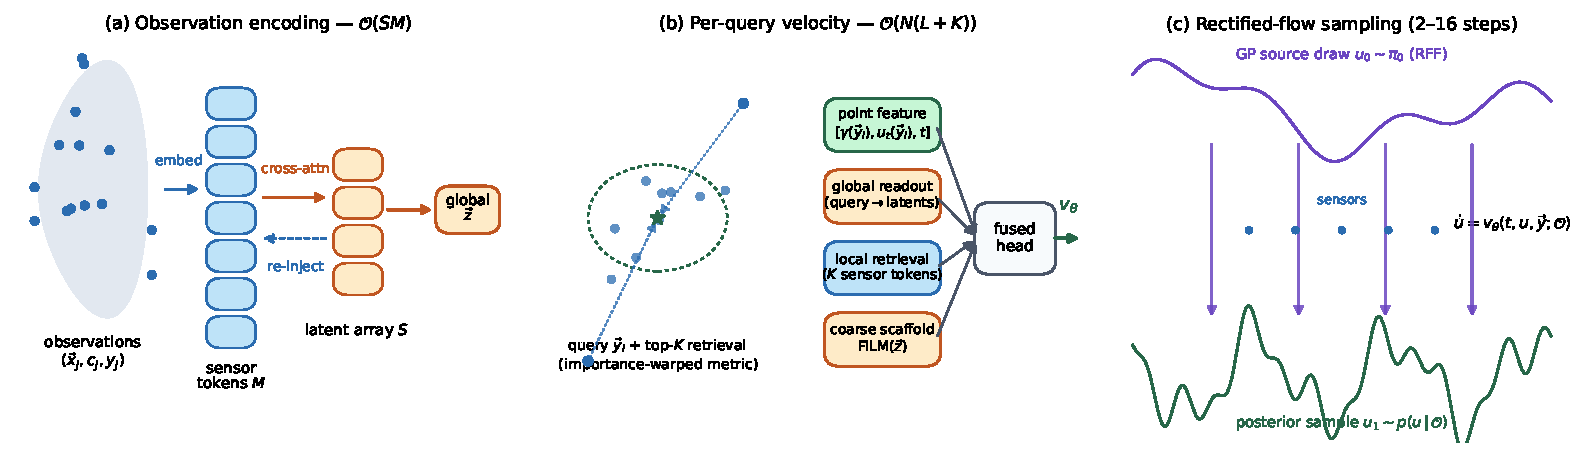
\includegraphics[width=0.56\linewidth]{figures/architecture.pdf}
\end{center}
\caption{\textbf{The \model{} architecture.} Sensor tokens are compressed by cross-attention into a small latent array (global pathway, $\gO(SM)$), which re-injects context back into the sensor tokens. Each query assembles its velocity from its point features, a readout from the latent array, and an importance-weighted retrieval over its $K$ nearest sensor tokens (local pathway, $\gO(NK)$). No dense volumetric representation is formed; cost is linear in the number of queries, and training estimates the loss on a random $\sim$2\% point subset per step.}
\label{fig:architecture}
\end{figure}

\subsection{Locality-factored conditioning}
\label{sec:method-arch}

The velocity network must expose the observations to every query point without incurring an all-to-all term in $N$ or a dense volumetric representation. \model{} factors the conditioning pathway by locality (Figure~\ref{fig:architecture}).

Each observation $(\vx_j,c_j,y_j)$ is embedded as a token from a Fourier positional encoding of $\vx_j$ \citep{tancik2020fourier}, the reading $y_j$, and a learned embedding of the quantity index $c_j$. A small array of $S$ learnable latents cross-attends to the $M$ sensor tokens \citep{jaegle2021perceiver} at cost $\gO(SM)$, refined by self-attention blocks that re-attend to the sensor tokens between rounds; the mean-pooled array provides a global summary, and a final pass writes that context back into the sensor tokens.

Each query $\vy_i$ then fuses three components: a point feature encoding its position, the current state $u_t(\vy_i)$, and $t$; a global readout cross-attending from a coordinate-conditioned decoder token to the latent array at cost $\gO(L)$; and a local retrieval over the $K$ nearest sensor tokens under the plain Euclidean metric (validity-masked), aggregated with softmax weights whose logits combine an RBF distance term with a learned, scaled per-sensor importance bias: $w_{ij}\propto\exp\!\big({-}\|\vy_i-\vx_j\|_2^2/2\sigma^2+s\,\beta_j\big)$. Neighbor selection is purely geometric; the bias $\beta_j$ reweights \emph{within} the retrieved neighborhood, letting informative sensors dominate it, which matters when sensing is anisotropic (surface-only layouts) or partially corrupted. A FiLM-modulated coarse prediction from the global summary enters as a gated residual, and a small MLP head produces the velocity. Retrieval and the $k$-nearest-neighbor search run as streaming kernel reductions \citep{charlier2021kernel}, so the $[N{\times}M]$ distance matrix is never materialized. Total cost per evaluation is $\gO(SM + NL + NK)$ with no term coupling query points to each other: compute is linear in $N$, and the same trained network evaluates on $10^{4}$ or $2\times10^{6}$ points unchanged.

\subsection{Training objective and sampling cost}
\label{sec:method-objective}

Two additions to \eqref{eq:loss} matter in practice. First, $t$ is drawn logit-normally, concentrating capacity at intermediate noise levels \citep{ma2024sit}. Second, generative models of turbulence exhibit spectral bias, reproducing large scales and attenuating the inertial range \citep{rahaman2019spectral}; following the observation that binned spectral penalties succeed where naive FFT losses do not \citep{chakraborty2026binned}, each batch appends a $32^3$ lattice block to the query set, and from the endpoint estimate $\hat{u}_1 = u_t + (1-t)\,v_\theta$ we penalize the squared difference of shell-averaged log power against $u_1$ over 12 radial bins, weighted by $t$. The total loss is $\gL_{\mathrm{FM}} + \lambda_{\mathrm{sp}}\gL_{\mathrm{sp}}$ with $\lambda_{\mathrm{sp}}=0.02$, and Section~\ref{sec:results-jhu} reports the resulting trade-off with $\lambda_{\mathrm{sp}}$ as the control.

At sampling time every quantity depending only on the observations and query coordinates---the sensor branch, the neighbor geometry, and the coordinate-conditioned readout---is computed at the first ODE step and reused exactly thereafter, so the marginal cost of a step falls to the fusion head: a full $125^3$ sample costs $4.5$\,s at 4 evaluations and $5.1$\,s at 16, making high-step operating points nearly free.

\paragraph{Amortized measurement operators.}
\label{sec:method-operators}
Conditioning is amortized by randomizing the measurement operator during training: each step draws the sensor count and layout afresh, and with configurable probability readings are corrupted with Gaussian noise of random amplitude, contiguous sensor regions are removed, and entire observed channels are dropped. The network thus learns one conditional velocity field over a family of operators, and at test time a single model serves that family without retraining or guidance; Section~\ref{sec:results-ops} additionally probes operators outside the training ranges. Known covariates (Mach, incidence) enter as parameter tokens exempt from corruption. Observed values can be enforced on the generated field at sampling time; we enforce for noiseless protocols and disable under sensor noise, where interpolating corrupted readings is undesirable. Training details are in Appendix~\ref{app:training}.

\section{Experiments}
\label{sec:results}

The experiments are organized around the asymmetry the method claims. Section~\ref{sec:results-scaling} measures the scaling separation that defines the regime: above $\sim$$300^3$, on unstructured discretizations, and under sensing geometries no grid can represent, ambient point-cloud generation is the only route that runs. Sections~\ref{sec:results-wing} and~\ref{sec:results-ops} then evaluate in that regime---surface-only sensing on unstructured wing meshes, and realistic corrupted operators on wildfire LES---where grid-based generative baselines can participate only after voxelization or resampling, if at all. Section~\ref{sec:results-jhu} closes with the converse control: a periodic, regular-grid turbulence benchmark chosen because it is the terrain voxel and patch methods are built for, where all ten baselines can compete at full strength and the comparison is fair by construction.

\paragraph{Evaluation protocol.}
Turbulence snapshots are strongly autocorrelated in time, and splitting consecutive DNS frames at random---standard practice---makes every validation frame a near-duplicate of a training frame (frame-to-frame correlation 1.00 at unit separation). Under such a split all methods, ours included, achieve errors two to three times lower, and the ranking measures interpolation rather than reconstruction. All turbulence results therefore use spatial holdout: training on three $125^3$ regions of the DNS, evaluation on a fourth, disjoint region, with temporally blocked splits inside the training set. Probabilistic metrics use $K{=}8$ ensembles on matched snapshots with identical seeded sensor draws for every method, compared by paired per-snapshot confidence intervals. Exact octahedral symmetry augmentation (48 signed axis permutations, discretization-exact on cubic grids) is supplied to every method. \todo{Temporally blocked same-region companion evaluation (retrains queued).}

\paragraph{Datasets.}
Three domains, each exposing one failure mode of existing methods (preprocessing in Appendix~\ref{app:datasets}). (i) Forced isotropic turbulence \citep{li2008public}: four disjoint $125^3$ cutouts of the $1024^3$ DNS ($1.95\times10^{6}$ points, velocity and pressure, 50 strided snapshots each), three for training and the fourth for evaluation. (ii) SHIFT-WING \citep{luminary2026shiftwing}: adaptively meshed RANS over transport-aircraft wing--fuselage variants at Mach 0.5--0.85; 673 cases (600/73), each $4\times10^{5}$ volume and $6.5\times10^{4}$ surface nodes carrying pressure and wall shear, geometry varying across cases and entering only through the observation point cloud. (iii) FireBench \citep{firebench2024}: wildfire LES at two wind speeds; we extract the fire-front region ($3.7\times10^{6}$ points; velocity, potential temperature, fuel density; 120 snapshots).

\paragraph{Baselines.}
We compare against the routes identified in Section~\ref{sec:intro}, configured for fairness rather than convenience (Appendix~\ref{app:baselines}). On the gridded benchmark, ten baselines, each audited for upstream fidelity before its numbers were admitted and parameter-matched to $6.5$M where the published configuration allows: the latent route (a parameter-matched 3D convolutional autoencoder with rectified flow in its latent space \citep[LDM-style;][]{rombach2022high}, standing in for the latent-diffusion family, and CoNFiLD \citep{du2024confild} in three arms with its published prior as the headline row), the voxel route (Gen4Turb \citep{oommen2026turbulent} at its native $120^3$; S3GM \citep{li2024s3gm}), a patchified-token route (SiT with a point tokenizer, ``SiT-point'' \citep{ma2024sit}), a spectral grid backbone inside our own framework (FNO3D), deterministic point methods (Senseiver \citep{santos2023senseiver}, DeepONet), and classical floors (nearest-neighbor, inverse-distance weighting, gappy POD, and the training mean). Upstream-faithful configurations are frozen; any tuned or enhanced variant is reported as a separately labelled arm. On the wing and wildfire experiments only the baselines whose interface honestly admits the data participate (point-native and grid-native respectively); the exclusions are stated per experiment rather than papered over.

\paragraph{Metrics.}
We report relative $L_2$ per channel as the primary accuracy metric---aggregates over channels are shown but flagged, since they average observed channels with unobserved ones that carry a different question---alongside single-sample relative $L_2$ (which measures whether individual realizations are physical rather than over-smoothed), band-resolved spectral ratios, fair CRPS \citep{gneiting2007strictly}, spread--error ratio, and central 90\% coverage, in per-field standardized units (Appendix~\ref{app:metrics}). Calibration metrics move with the operating point by more than they separate methods---raising NFE from 4 to 16 shifts our spread--error by $+0.22$, and enlarging ensembles from $K{=}8$ to $32$ shifts coverage by $+0.11$---so every calibration number in this paper carries its operating point (sensor density, NFE, $K$, checkpoint) and cross-method comparisons are made only at matched settings. One limit of the protocol should be stated plainly. Forward statistical computation can construct a conditional ground truth by re-running a solver from micro-perturbed states and comparing distributions at a fixed condition \citep{raonic2026gencfd}; reconstruction admits no such construction, since each sensor draw has exactly one realization behind it. Our calibration is therefore empirical---measured across held-out snapshots and randomized observation operators---rather than against a many-member conditional ensemble.

\subsection{The cost of resolution}
\label{sec:results-scaling}

\begin{figure}[tbp]
\begin{center}
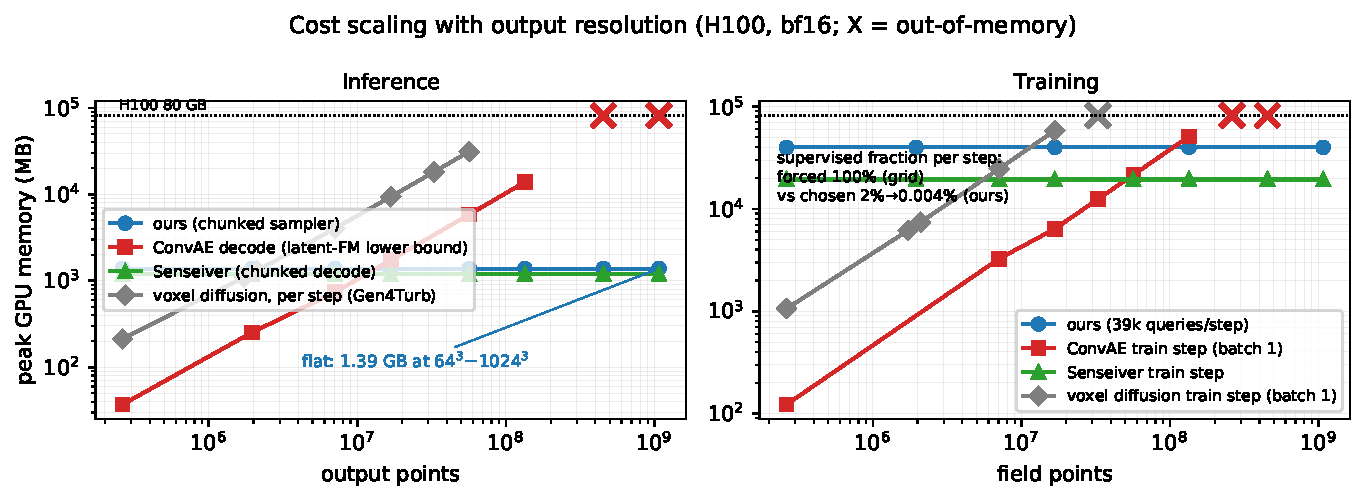
\includegraphics[width=0.99\linewidth]{figures/scaling_cost_mem.pdf}
\end{center}
\caption{\textbf{Measured peak memory versus output resolution} (H100, bf16, log--log; OOM markers are measured failures, not extrapolations), for full-field sampling (left) and training steps (right). Grid methods (voxel diffusion, convolutional AE) scale cubically and fail at $320^3$ and $640^3$; point methods (\model{}, Senseiver) are flat to $1024^3$ ($10^9$ points). The annotation gives the fraction of the field supervised per training step: 100\% forced for grid methods, a fixed 39k-point budget for \model{} (2\% at $125^3$, 0.004\% at $1024^3$). Wall-clock panels are in Figure~\ref{fig:scaling-full}.}
\label{fig:scaling}
\end{figure}

Figure~\ref{fig:scaling} reports measured peak memory and wall-clock for training steps and full-field sampling from $64^3$ to $1024^3$; every out-of-memory marker is an observed failure on an 80\,GB H100. The axis separates two computational families. Grid methods scale cubically: the convolutional autoencoder anchoring the latent baseline trains at $50.9$\,GB for one $512^3$ field and fails at $640^3$ at batch size 1 (at production batch size the wall falls between $256^3$ and $320^3$), and the voxel diffusion model fails at $320^3$ at batch size 1 while already consuming $57.5$\,GB at $120^3$. Point methods are flat: \model{} trains at $39.9$\,GB and $0.44$\,s per step and samples at $1.4$\,GB peak at every resolution tested, and Senseiver shares the profile ($19.4$\,GB train, $1.2$\,GB inference)---flatness is a property of point computation, not of our model alone. Within that family \model{} is the only generative member; the deterministic one pays a factor of two on observed-channel accuracy at matched sensing (0.361 vs.\ 0.176 relative $L_2$, Table~\ref{tab:jhu}) and cannot produce an ensemble.

The annotations give the mechanism: a voxel or convolutional model is structurally committed to supervising every grid cell at every step---its memory is the supervision---whereas \model{} chooses its budget independently of resolution, and the query-budget ablation (Section~\ref{sec:results-jhu}, Appendix~\ref{app:extra}) shows that budget saturates. The honest converse is that grid computation is cheaper below the crossover ($\sim$$240^3$ for inference): a convolutional decode of a $125^3$ field costs 6\,ms where our chunked point evaluation costs 4.5\,s. Stated precisely, the claim is constant memory with respect to the output discretization and linear-time inference, not constant total cost; the regime where \model{} is the only option is the one the applications occupy---resolutions above $\sim$$300^3$, unstructured discretizations, and sensing geometries no grid can represent. The constancy of the training graph also raises the right follow-up question, whether the model trained at one discretization transfers as a function-valued sampler to finer and irregular ones; a direct discretization-transfer experiment (training at $125^3$, reconstructing a native $500^3$ cutout and irregular subsets of it) is in preparation as a core test of the function-space claim. \todo{Discretization-transfer experiment: $125^3$-trained model evaluated on a $500^3$ JHTDB cutout and on irregular/coarsened point sets, with convergence of spectra and error across discretizations.}

\subsection{Native geometry: surface-only sensing on unstructured wing meshes}
\label{sec:results-wing}
The wing exercises the two capabilities that motivated the method and that no grid-based generative model has: an unstructured mesh whose geometry changes across cases, and observations confined to the body surface. This experiment is where the asymmetry of Section~\ref{sec:results} becomes concrete. Voxel diffusion, patchified transformers, and latent-grid flow matching cannot be trained here without first resampling the adaptive mesh onto an axis-aligned grid---a lossy preprocessing step that erases exactly the near-wall resolution the mesh exists to provide---so their rows are reported as \emph{not applicable without resampling} rather than silently omitted. Point-native methods can compete fairly, and do: Senseiver conditions on the same surface sensor set, and CoNFiLD-class latent neural fields are point-native by construction. \todo{Wing baseline table: \model{}, Senseiver (trained), latent FM (trained; grid-latent---label its resampling honestly), CoNFiLD, gappy POD, SiT-point, with ``n/a without resampling'' rows for Gen4Turb/S3GM/FNO3D; runs and gaps inventoried in \texttt{GAP\_ANALYSIS\_WING\_FIREBENCH\_2026-08-30.md}.}

From 640 surface sensors (512 pressure taps, 128 shear gauges, with Mach and incidence as parameter tokens), \model{} recovers the volumetric pressure-coefficient field on 8 held-out geometries at 0.126 relative $L_2$ and velocities at 0.53--0.69 (CRPS 0.18, spread--error 0.68, coverage 0.38; $K{=}4$, NFE 4), with predictive standard deviation concentrating in the boundary layer and wake---the regions genuinely undetermined by surface data (Figures~\ref{fig:qual-wing},~\ref{fig:unc-wing}). Three pathways could carry surface information to off-body queries: the $k$-nearest retrieval, which returns each query's nearest surface sensors regardless of absolute distance (selection is purely Euclidean, and the softmax weights are normalized within the neighborhood); the learned importance bias, which reweights sensors within that neighborhood; and the global summary, which every query reads. Which pathway is load-bearing off-body is a hypothesis we test by ablation rather than assert. \todo{Pathway ablation (global-only / local-only / importance bias off), tap-count sweep, slice gallery.}

\subsection{Realistic measurement operators: noise, occlusion, and channel dropout}
\label{sec:results-ops}

\begin{table}[tbp]
\caption{Wildfire LES ($3.7$M points, 5 fields) under realistic measurement operators (relative $L_2$ of ensemble mean / fair CRPS; $K{=}8$, 8 snapshots, identical seeded operator realizations for all methods). Sensors observe the three wind components at $\sim$1\% of points. \model{} is a single amortized model across all rows.}
\label{tab:ops}
\begin{center}
\footnotesize
\setlength{\tabcolsep}{4.5pt}
\begin{tabular}{lcccccc}
\toprule
& \multicolumn{2}{c}{\model{}} & \multicolumn{2}{c}{Latent FM} & \multicolumn{2}{c}{Senseiver} \\
\cmidrule(lr){2-3}\cmidrule(lr){4-5}\cmidrule(lr){6-7}
Operator & Rel.\ $L_2$ & CRPS & Rel.\ $L_2$ & CRPS & Rel.\ $L_2$ & CRPS \\
\midrule
Clean & \textbf{0.456} & \textbf{0.234} & 0.724 & 0.356 & 0.779 & 0.443 \\
Noise $\sigma{=}0.1$ & \textbf{0.458} & \textbf{0.237} & 0.722 & 0.355 & 0.779 & 0.444 \\
Noise $\sigma{=}0.3$ & \textbf{0.461} & \textbf{0.248} & 0.724 & 0.356 & 0.779 & 0.445 \\
Slab occlusion (25\%) & \textbf{0.511} & \textbf{0.275} & 0.720 & 0.355 & 0.780 & 0.443 \\
Channel dropout ($u$ only) & \textbf{0.603} & \textbf{0.355} & 0.719 & 0.309 & 0.908 & 0.514 \\
\bottomrule
\end{tabular}
\end{center}
\end{table}

Table~\ref{tab:ops} evaluates the second deployment regime, on wildfire LES at $3.7$M points: sensing that is noisy, occluded by the phenomenon being measured, and missing channels. The extraction is a regular LES crop, so unlike the wing this experiment does not exclude grid methods by geometry---the baselines here (the latent route and Senseiver) participate on their native terms, and the comparison isolates the operator realism axis alone. \todo{FireBench baseline coverage: latent FM and Senseiver rows exist; assess adding one voxel-diffusion row (Gen4Turb-class) for route completeness --- see gap analysis.} One amortized \model{} wins every cell, with qualitative margins: $0.3\sigma$ sensor noise costs one percent relative, removing a 25\% slab of sensors twelve percent, and dropping two of three wind components a third. Its worst case (0.603) still beats either baseline's best case under clean, complete observations (0.719 and 0.779). One row is genuinely out of distribution---training used noise amplitudes up to $0.1\sigma$, so the $0.3\sigma$ row is triple anything seen---while the occlusion and dropout rows lie inside the amortized family, demonstrating robustness within a deliberately broad operator distribution rather than extrapolation. \todo{Add further OOD operators: ball occlusion, sensor density outside the training range, structured arrays.}

The baselines' apparent stability across rows deserves the correct reading: their numbers barely move because they are bias-dominated, and a model that extracts little of the information in the sensors loses little when that information is corrupted. The latent baseline reconstructs at 0.72 relative $L_2$ under every operator (predicting the zero field scores 1.0), and its CRPS improves under channel dropout only because its spread is large where its mean is wrong. \model{}'s errors respond to the information content of the observations because the model uses that information; graceful, monotone degradation, not invariance, is the behavior a practitioner should want. The latent baseline's dispersion ratio here (0.87) exceeds ours (0.76), but at more than twice the CRPS; the proper score, integrating both, favors \model{} by 34\% in every condition. A clean-trained control isolates what operator amortization actually buys: trained without any corruption, the control matches the robust model under noise and slab occlusion (0.458 vs.\ 0.461 at $0.3\sigma$; 0.513 vs.\ 0.511 under occlusion)---robustness to those perturbations comes from the conditioning architecture, not the training distribution---but collapses under channel dropout (0.743 vs.\ 0.603), the one operator that changes the structure of the observation set. Amortized operator training is what covers that structural shift, and it costs nothing in the clean condition (0.455 vs.\ 0.456).

Cross-variable inference falls out of the same interface: observing only wind, the model recovers unobserved fuel density at 0.044 relative $L_2$ and potential temperature at 0.49, degrading only to 0.064 and 0.52 when two of the three wind components are also removed (Appendix~\ref{app:extra}). The randomized observed-channel embedding is what makes a wind-only, single-component operator an interpolation rather than an extrapolation for the conditioning network. The uncertainty is placed where the physics is ambiguous rather than uniformly: averaged over the hottest 5\% of the domain the predictive standard deviation is $7$--$25\times$ its value in the ambient half (for potential temperature, $1.32$ against $0.05$), and Figure~\ref{fig:qual-fb} shows it tracing the fire front in the fuel bed, which the model never observes.

\subsection{The controlled benchmark: gridded turbulence with the full fleet}
\label{sec:results-jhu}

This section is the fairness control. A periodic $125^3$ cutout is exactly the terrain voxel, patchified, and latent-grid methods are built for---nothing about the discretization disadvantages them---so it is where their comparison against \model{} is most informative and least favorable to us. We report it in full.

\begin{table}[tbp]
\caption{Gridded isotropic turbulence, spatially disjoint evaluation region ($1.95$M points; $U_x,U_z$ observed at 1\% of points per channel, $U_y^*,p^*$ unobserved; canonical seeded sensor draws, all $n{=}50$ held-out snapshots, $K{=}8$ ensembles at each method's listed sampler setting, best-checkpoint policy per Appendix~\ref{app:baselines}). Per-channel relative $L_2$ of the ensemble mean is primary; agg$^\dagger$ averages all four channels and is flagged, not headlined. Unobserved-channel error $\ge 1.0$ means worse than predicting the training mean; values near 1.0 across the fleet reflect a shared identifiability limit of point-conditioned methods, not per-method defects. Spread--error and coverage ideals are 1.0 and 0.90; deterministic methods: CRPS reduces to MAE, dispersion undefined. Step budgets are as-run, not equalized: every external baseline received at least our 48k optimizer steps except SiT-point (wall-clock-matched, 38.5k); CoNFiLD trains on a wall-clock budget. Labelled improvement arms (Senseiver capacity, DeepONet++ structured branch, CoNFiLD repairs, S3GM normalized guidance) are reported separately. \todo{S3GM canonical row and improvement-arm rows: origin evals finalizing.}}
\label{tab:jhu}
\begin{center}
\footnotesize
\setlength{\tabcolsep}{3.4pt}
\begin{tabular}{lcccccccc}
\toprule
Method & $U_x$ & $U_y^*$ & $U_z$ & $p^*$ & agg$^\dagger$ & CRPS & Spr/Err & Cov.$_{90}$ \\
\midrule
\model{} (NFE 4) & 0.176 & 1.048 & 0.182 & 0.964 & 0.593 & 0.291 & 0.63 & 0.54 \\
Latent flow matching & 0.248 & \textbf{0.727} & 0.257 & \textbf{0.646} & \textbf{0.469} & \textbf{0.244} & 0.68 & 0.56 \\
SiT-point ($N{=}32$) & \textbf{0.143} & 0.968 & \textbf{0.132} & 0.937 & 0.545 & 0.338 & 0.75 & 0.58 \\
FNO3D (our framework, NFE 4) & 0.188 & 0.904 & 0.191 & 1.061 & 0.586 & 0.269 & \textbf{0.94} & \textbf{0.63} \\
CoNFiLD (published prior, DPS 1000) & 0.409 & 0.751 & 0.374 & 1.007 & 0.635 & 0.371 & 0.82 & 0.57 \\
Gen4Turb (anneal, 32-step) & 0.224 & 0.996 & 0.455 & 1.005 & 0.670 & 0.407 & 0.37 & 0.33 \\
S3GM (JHU-tuned, $N{=}200$) & \multicolumn{8}{c}{\todo{canonical eval finalizing}} \\
\midrule
Senseiver (deterministic) & 0.361 & 1.077 & 0.380 & 0.978 & 0.699 & 0.479 & --- & --- \\
DeepONet (deterministic) & 0.593 & 0.972 & 0.652 & 0.985 & 0.800 & 0.570 & --- & --- \\
\midrule
Nearest neighbor (KD-tree) & 0.209 & 1.000 & 0.219 & 1.000 & 0.607 & 0.406 & --- & --- \\
IDW ($k{=}8$, non-periodic) & 0.174 & 1.000 & 0.181 & 1.000 & 0.589 & 0.396 & --- & --- \\
Gappy POD ($r{=}80$) & 0.523 & 1.306 & 0.540 & 1.443 & 0.953 & 0.673 & --- & --- \\
Training mean & 1.000 & 1.000 & 1.000 & 1.000 & 1.000 & 0.786 & --- & --- \\
\bottomrule
\end{tabular}
\end{center}
\end{table}

Table~\ref{tab:jhu} reports the full fleet, and the honest headline is that no method leads every column. SiT-point posts the best observed-channel errors (0.143/0.132) at roughly $150$\,s per field---239 sequential 8{,}192-token chunks at 32 steps---and its single samples carry chunk-incoherent speckle that the ensemble mean averages away (member-level statistics below). The latent flow-matching baseline leads the aggregate, the unobserved channels, and CRPS (0.469; $U_y$ 0.727, $p$ 0.646): its convolutional decoder emits globally structured fields even where no sensor constrains them, at the dissipation-range price quantified below. Non-periodic inverse-distance weighting---a training-free interpolant---edges our observed-channel error (0.174 vs.\ 0.176 on $U_x$), so we do not claim to beat interpolation on observed channels at 1\% density; the generative payoff concentrates where the problem is ill-posed: unobserved channels, corrupted operators (Section~\ref{sec:results-ops}), and sparser sensing.\todo{Density-sweep/Pareto figure (accuracy vs.\ inference cost vs.\ train GPU-h, with sensor density): generative wins at 0.1\%, interpolation at 10\%; numbers in FLEET\_SUMMARY\_TABLE.} What \model{} owns at this operating point (1\%, NFE 4, $K{=}8$, best checkpoint): observed-channel accuracy within 0.033 relative $L_2$ of the leader while sampling in 4 network evaluations against 32--1000 for the guided-diffusion and transformer baselines, the strongest member-level dissipation-range fidelity of the generative fleet, and a predictive uncertainty characterized and repaired below. \todo{Paired per-snapshot CIs vs.\ SiT-point and latent FM from the canonical $n{=}50$ JSONs; training-seed replicates (2--3 seeds) for our row.}

Two knobs expose a distortion--dispersion frontier (Appendix~\ref{app:extra}, Tables~\ref{tab:spectral}--\ref{tab:nfe}). Step count: two evaluations give the sharpest single samples, four are the CRPS optimum, and dispersion rises monotonically with further steps at flat CRPS, which the per-solve conditioning cache makes nearly free. Spectral weight: raising $\lambda_{\mathrm{sp}}$ from 0 to 0.02 improves single-sample error and inertial-band fidelity at a measured cost in spread, and at 0.05 the accuracy gain saturates while dispersion degrades further. We report $\lambda_{\mathrm{sp}}{=}0.02$ as the primary model; no single point on the frontier is best for every use.

Two confounds are closed by ablation (Appendix~\ref{app:extra}): doubling the per-step query budget from 2\% to 4\% does not improve held-out loss (three seeds), so subsampled supervision is not the binding constraint even though the latent baseline consumes roughly $50\times$ more supervised values per step; and octahedral augmentation is the operative one, with continuous rotations, translations, and proper-rotation restrictions all inside run-to-run variance.

\begin{figure}[tbp]
\begin{center}
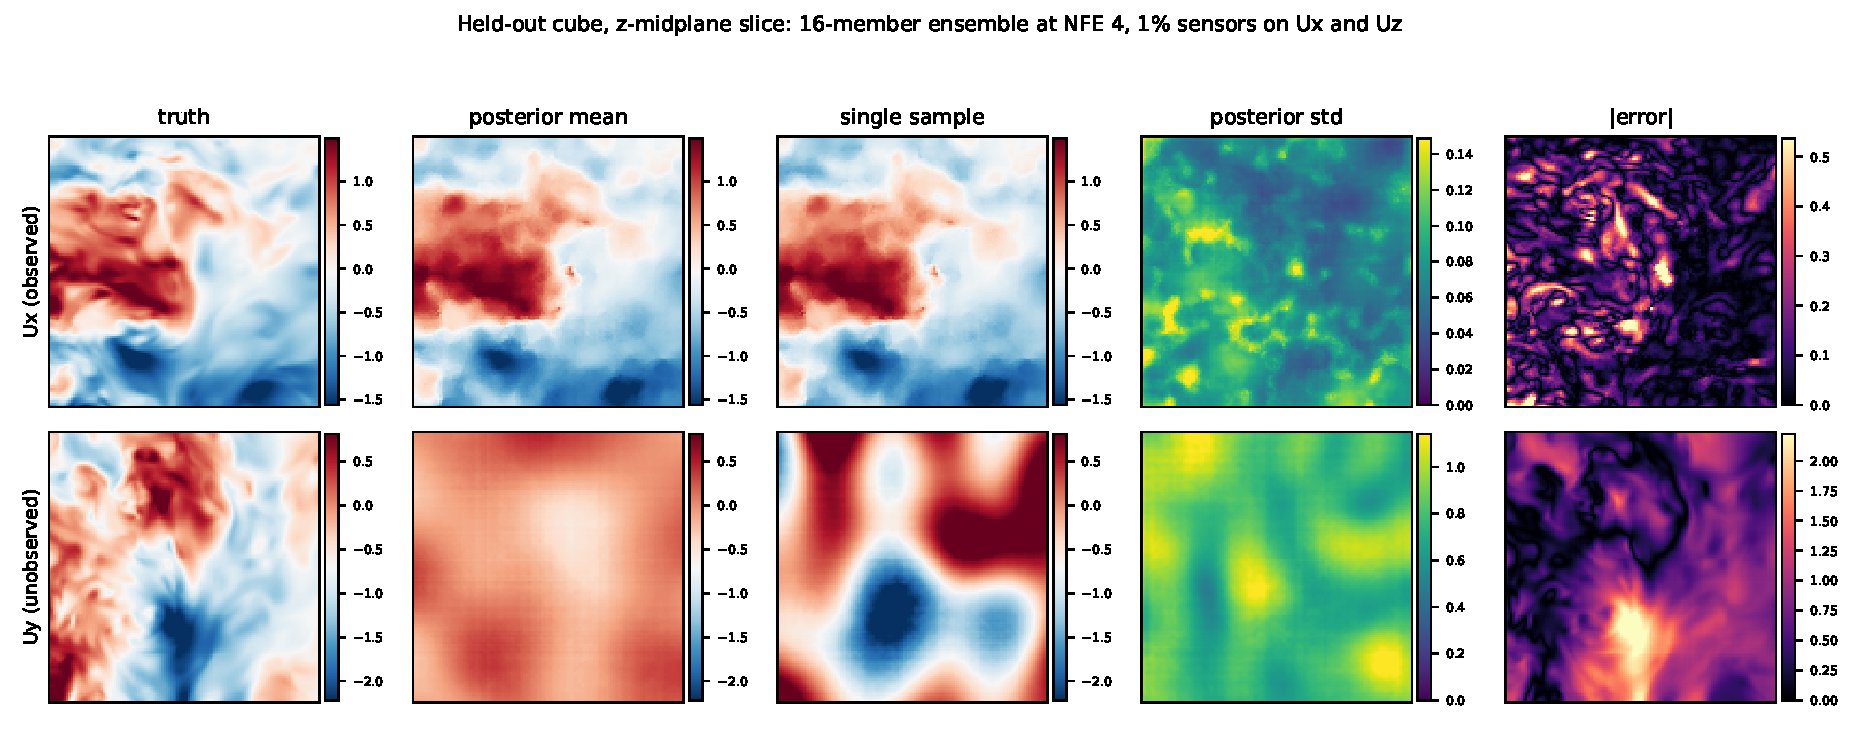
\includegraphics[width=0.94\linewidth]{figures/qual_jhu.pdf}
\end{center}
\caption{\textbf{Reconstruction and uncertainty on the held-out cube} ($z$-midplane slice, 16-member ensemble at NFE 4, 1\% sensors on $U_x$ and $U_z$). Top: an observed channel, recovered sharply, standard deviation an order of magnitude below the field scale. Bottom: $U_y$, which no sensor constrains---the ensemble mean collapses toward the prior mean while individual samples stay sharp and the standard deviation rises to the field scale, so the model reports that it does not know. The $|$error$|$ column tracks the standard-deviation column throughout (pointwise correlation 0.60).}
\label{fig:qual}
\end{figure}

\paragraph{What the uncertainty tracks.} Figure~\ref{fig:qual} shows the reconstruction and its spread directly; Appendix~\ref{app:extra} adds pointwise diagnostics. The predictive standard deviation separates the channels the sensors constrain from those they do not: on the observed $U_x$ it averages $0.09$ against RMS error $0.17$, while on the unobserved $U_y$ it rises to $0.87$ against RMS error $0.95$. Two structural findings complete the characterization (all at $K{=}8$, best checkpoint). First, the spread--error relation is monotone but above the diagonal, the pointwise form of the underdispersion the aggregate metrics report. Second, the spread does respond to distance from the nearest sensor---the profile grows away from the data---but it never sharpens below a hard floor of ${\approx}0.09$ in standardized units, even at sensor locations, and the profile is density-invariant: expressed against distance, the same curve holds from 0.1\% to 1\% sensor coverage. Raising NFE from 4 to 16 rescales the entire profile by ${\approx}1.5\times$ without changing its shape. The consequence is that no (density, NFE) operating point is calibrated out of the box---spread--error runs from 0.44 to 1.56 across densities---but the miscalibration has a known, low-dimensional mechanism: a distance-indexed profile with a floor, rescaled by the sampler setting.

\paragraph{From characterized to repaired: post-hoc recalibration.}
\label{sec:results-recalib}
That mechanism makes the uncertainty repairable. We recalibrate post hoc under a strict split discipline: all fitting uses the odd-index tuning half of the held-out snapshots; every reported number is frozen on the even-index test half. Two estimators, in order of strength: (i) a per-density (optionally per-channel) scalar spread multiplier fitted to spread--error $=1$ on the tuning split; (ii) conformalized quantile scaling in which per-point ensemble intervals are rescaled by a conformal quantile fitted per distance-to-nearest-sensor bin---distance being the profile's sufficient statistic---which carries a finite-sample marginal coverage guarantee on exchangeable points. Three honesty requirements govern the reporting: the repair is post hoc and stated as such; it rescales stated uncertainty and cannot sharpen the ${\approx}0.09$ floor, which remains the residual limitation; and the identical wrapper is offered to the generative baselines (latent flow matching at minimum), so the comparison is not one-sided. \todo{TEST-split spread--error and coverage curves before/after for both estimators, ours and latent FM, at 2--3 densities (fits: \texttt{src/recalibrate\_spread.py}, \texttt{src/conformal\_recalib.py}; per-point dumps queued on origin).}

\paragraph{Small-scale fidelity.} Energy spectra, structure functions and velocity-gradient PDFs of single samples (Figure~\ref{fig:spectra}, Appendix~\ref{app:extra}) test the premise behind avoiding an autoencoder. One estimator detail is load-bearing, so we state it first: the cutouts are sub-blocks of a larger DNS and are not periodic, so an unwindowed FFT spreads the edge discontinuity into a broadband floor. On our data the raw spectrum of the \emph{truth} falls only $2.4\times$ between $k{=}32$ and the Nyquist wavenumber, and a deliberately smooth Gaussian-process draw---whose energy there is zero to machine precision---registers the same floor. A variance-preserving Hann taper restores a $5.8\times10^{5}$ decay and reduces that same draw to $5\times10^{-5}$ of the DNS inertial-range energy. Ratios computed without the taper are ratios of two floors and tend to unity for every method; all spectral numbers we report use the windowed estimator. Spectral recovery also does not compare across conditioning problems: \citet{raonic2026gencfd} resolve spectra at $128^3$ from initial and boundary data that determine the flow, whereas our operators supply on the order of one percent of the domain and leave whole channels unobserved. For a channel no sensor constrains, the realization's small scales are not recoverable even in principle---only their statistics are---so we read our own spectral shortfall against that ceiling rather than against theirs.

Measured this way the comparison splits by band and neither model is uniformly better. The latent baseline holds more inertial-range energy than \model{} ($0.62$ vs.\ $0.41$ for $U_x$ over $k\in[8,31]$) but collapses in the dissipation range, retaining $0.07$--$0.09$ of the DNS energy over $k\in[32,45]$ against our $0.40$--$0.46$: the autoencoder spectral floor \citep{rafiq2026spectrally,glaws2020deep} appearing where it was predicted. Our own high-wavenumber content is not recovered turbulence either---the spectrum flattens into a plateau instead of continuing to decay, the signature of broadband noise, reaching $3.5$--$4.8\times$ the DNS energy on pressure. Ambient generation therefore avoids the compression floor at the smallest scales while under-producing the inertial range, latent compression does the opposite, and neither reproduces the DNS spectrum from 1\% sensors; Appendix~\ref{app:extra} localizes our deficit to the channels the sensors do not constrain.

\section{Conclusion}
\label{sec:conclusion}

Generative reconstruction of 3D fields has been blocked not by modeling capacity but by a structural mismatch: generative architectures compute globally on dense discretizations, while the problem is defined on scattered points and needs only local and summary information at each. \model{} resolves it by carrying rectified flow directly on field values with a Gaussian-process source, locality-factored conditioning, and subsampled function-space training. The measured consequences: costs flat from $64^3$ to $1024^3$ where voxel and autoencoder pipelines fail at $320^3$--$640^3$; volumetric predictive distributions from surface-only sensors on varying unstructured geometries, and uniform dominance under corrupted sensing at $3.7$M points---the deployment regimes grid-based generative methods cannot enter; and, on the controlled gridded benchmark where ten audited baselines compete at full strength, observed-channel accuracy within 0.033 of the per-column leader at a fraction of its sampling cost, the strongest member-level dissipation-range fidelity of the generative fleet, and the only predictive uncertainty in the comparison that is characterized mechanistically and repaired post hoc under a tune/test split. \model{} reconstructs single snapshots; the natural extension is to condition on sensor time histories with an explicit lead time, training over all observation-to-target time pairs so that one model serves both instantaneous reconstruction and forward statistical prediction, as the semigroup structure of the flow map permits \citep{raonic2026gencfd}.

Limitations are equally measurable. Raw coverage sits below nominal at the primary operating point (0.54 against 0.90 at 1\%, NFE 4, $K{=}8$), and while the post-hoc repair restores stated coverage on the test split, the ${\approx}0.09$ spread floor is a property of the trained model that recalibration cannot remove; on the gridded benchmark's observed channels a training-free interpolant is marginally more accurate at 1\% density; single-snapshot reconstruction ignores temporal information that assimilation exploits; per-domain training is still required; and constant-memory inference pays a linear time cost, making \model{} the slowest method in absolute terms at large resolution (41 minutes for a $10^9$-point sample). Sharpening calibration, conditioning on sensor time histories, and pretraining across flow families are the natural continuations.

\label{endconclusion}
\subsection*{Reproducibility statement}
All experiments use publicly available data: the JHTDB isotropic turbulence database, the SHIFT-WING dataset (CC-BY-NC-4.0), and the public FireBench store; exact cutout indices, crop definitions, subsampling seeds, and normalization are specified in Appendix~\ref{app:datasets}. Architecture and training hyperparameters for \model{} and all baselines are listed in Appendices~\ref{app:architecture}--\ref{app:baselines} together with the configuration files used for every run. Code, configurations, and dataset preparation scripts will be released. \todo{Anonymous code link at submission.}

\subsection*{AI use statement}
\todo{Complete per ICLR 2027 policy before submission: disclose the use of AI assistance for literature search, code development, and manuscript drafting, with author verification of all content.}

\bibliography{references}
\bibliographystyle{iclr2027_conference}

\appendix

\section{Architecture details}
\label{app:architecture}

The velocity network used for all experiments has $6.51$M trainable parameters (parameter-matched to the latent flow-matching baseline's two stages combined). Sensor tokens and queries use Fourier positional encodings with 32 bands and maximum frequency 64. The global pathway compresses $M$ sensor tokens into $S{=}128$ latents of width 256 with 8-head cross-attention, refined by 4 latent self-attention blocks with feed-forward multiplier 4; sensor re-injection cross-attention runs after every block, and a final back-attention pass writes latent context into the sensor tokens. The per-query readout attends from a coordinate-conditioned decoder token to the latent array. The local pathway gathers the $K{=}16$ nearest sensor tokens under the Euclidean metric and aggregates them with the importance-biased softmax of Section~\ref{sec:method-arch} with a learnable RBF bandwidth; a training-time ablation on a trained checkpoint found $K{=}64$, 32, and 16 indistinguishable in reconstruction error (relative $L_2$ 0.273/0.273/0.272), so the smallest is used. Neighbor search and RBF aggregation run as streaming KeOps reductions \citep{charlier2021kernel} with query chunking (2{,}048 queries per chunk for the global readout, 4{,}096 for decoding). The source GP uses 256 random Fourier features with correlation length 0.15 in normalized coordinates.

Two implementation details matter at our scale. First, cross-attention over tens of thousands of variably valid sensor tokens with a key-padding mask forces the memory-efficient (CUTLASS) attention backward, which at $M{\approx}39$k keys is $\sim$70$\times$ slower at the kernel level than the flash backward; selecting each item's valid keys by boolean mask and running unmasked attention per item is mathematically identical (max deviation $4\times10^{-6}$) and doubles training throughput ($0.88\to0.41$\,s per step, compiled). Second, during ODE sampling, all sensor-branch activations, neighbor geometry, and the coordinate-conditioned readout are cached after the first step (Section~\ref{sec:method-objective}); the cache is exact (bitwise-zero output difference) and reduces a 16-step $125^3$ solve from 69.5\,s to 5.1\,s.

\section{Training details}
\label{app:training}

All models train on single 80\,GB H100 GPUs in bf16 autocast with an exponential moving average of weights (decay 0.9995) used for evaluation, Adam at learning rate $10^{-4}$, weight decay $10^{-6}$, and batch size 20 point-cloud samples. Turbulence: 6{,}000 epochs ($\sim$20\,h wall-clock; the latent baseline's two stages total $\sim$21\,h, so total budgets are matched), 39{,}062 query points per sample per step, per-channel sensor counts drawn uniformly on integers between 0.1\% and 1\% of points, observed channels $\{U_x,U_z\}$, $t$ logit-normal, $\lambda_{\mathrm{sp}}{=}0.02$ with a $32^3$ spectral block and 12 bins. Wildfire: 3{,}500 epochs, observed channels $\{u,v,w\}$, sensor counts 0.03--1\%, operator amortization with noise amplitude up to $0.1\sigma$, slab occlusion probability 0.2, and observed-channel dropout probability 0.3; lateral-reflection augmentation. Wing: 4{,}000 epochs, surface pool of 512 pressure + 128 shear sensors drawn per step from the $6.5\times10^4$-node skin, Mach and incidence tokens, spanwise-reflection augmentation. The forward pass is compiled; compilation preserves checkpoint compatibility.

\section{Datasets and preprocessing}
\label{app:datasets}

\paragraph{Isotropic turbulence.} Four $125^3$ cutouts at disjoint spatial locations of the JHTDB \texttt{isotropic1024coarse} DNS, 50 snapshots each at a stride of 100 database steps, fields $(U_x,U_y,U_z,p)$, per-field standardized. Training uses cutouts 1--3 (150 snapshots); all reported evaluation uses cutout 4. Within the training cutouts, temporal blocks are kept contiguous. The leakage analysis motivating this protocol (Section~\ref{sec:results}) was run on 617 consecutive frames of a single cutout: frame-to-frame correlation is 1.00 at unit separation and 0.67 at separation 100, and a shuffled split placed every validation frame within one frame of a training frame.

\paragraph{SHIFT-WING.} 673 converged RANS cases spanning the dataset's Mach blocks (0.5--0.85), incidence 0.02--3.99$^\circ$, and 40 geometry parameters (aspect ratio 7.5--11, sweep 25--37$^\circ$). Each case is reduced to $4\times10^5$ near-body volume nodes (subsampled from the adaptive mesh) and the full $6.5\times10^4$-node surface pool carrying $C_p$ and the three wall-shear components as distinct observed-quantity indices; Mach and incidence enter as parameter tokens with dedicated indices. Split 600/73 by case; physical-coordinate spanwise reflection augments training.

\paragraph{FireBench.} From the public FireBench store, the two LES runs at 10 and 12\,m/s driving wind. The 3D extraction crops a $152\times126\times192$ region around the fire front (streamwise 250--706\,m at 3\,m, full lateral extent at 2\,m, 0--192\,m altitude at 1\,m), avoiding the empty sky aloft, with fields $(u,v,w,\theta,\rho_f)$; 60 snapshots per run at stride 2, merged to 120, temporally blocked split with a 10-frame guard gap.

\section{Baseline configurations}
\label{app:baselines}

\paragraph{Latent flow matching.} A 3D convolutional autoencoder (3 levels, $\sim$$16^3\times48$ latent) trained on full fields, followed by rectified flow in the latent space with a point-encoder conditioning branch over the identical sensor draws; combined parameter count 6.68M ($+2.7$\% vs.\ ours). Identical data, splits, augmentation, and sensor protocol. Two disclosures: a conditioning defect found in audit was repaired before the reported numbers (the repaired arm is the one in Table~\ref{tab:jhu}), and its optimizer budget (209k flow steps $+$ 95k autoencoder steps) exceeds ours by roughly $6.3\times$, reported as run rather than equalized. The two-stage structure gives this baseline roughly $50\times$ more supervised field values per step than \model{}; the supervision ablation in Appendix~\ref{app:extra} addresses the resulting confound.

\paragraph{Gen4Turb.} The released code and architecture of \citet{oommen2026turbulent} (elucidated-diffusion U-Net, channel dimension 16, self-conditioning, mask-channel conditioning), trained on our turbulence data at its native $120^3$ crop of the $125^3$ region, with $\sigma_{\mathrm{data}}$ taken from its own preprocessing. Its training script defaults to a compute budget an order of magnitude beyond every other method; we checkpoint every 10 epochs and report the wall-clock-matched checkpoint (epoch 4{,}930, matching our 20\,h). Two observation protocols are evaluated: its native shared-mask protocol (all four channels observed at the same 1\% locations; more information than any other method receives) and our strict protocol (two channels at independent locations). Because the strict protocol is out of distribution for the shared-mask training, we additionally retrained it under our exact observation model (independent per-channel masks, coverage drawn 0.1--1\%); the retrain moved strict-protocol accuracy by less than 0.01 (0.700$\to$0.706), and its validation-selected checkpoint is substantially worse than the budget-matched one (0.921 vs 0.706), so the table reports the budget-matched retrained model, the choice most generous to the baseline. The reported arm adds one labelled learning-rate-anneal line to otherwise untouched upstream code (105k steps, 32 denoising steps). \todo{Refresh this paragraph against the 2026-08-29 fleet audit: best checkpoint moved (ep3081), and the retrain-delta numbers here predate the audited run---re-source from the canonical $n{=}50$ JSONs.}

\paragraph{Senseiver.} The attention-based deterministic reconstructor of \citet{santos2023senseiver} under identical sensor randomization, augmentation, and splits, trained to its own convergence ($\sim$79k steps). As a deterministic model its CRPS equals its MAE, and no dispersion metrics apply. Its reconstructions are severely low-passed with unobserved channels at climatology---the global-latent-bottleneck signature, not a training failure (validation descended to its optimum under patience-based stopping). A capacity sweep (128/256/512 latent tokens) is reported as a labelled arm. \todo{Register Senseiver capacity-arm results when origin evals land.}

\paragraph{SiT-point.} SiT \citep{ma2024sit} with a point tokenizer (not patchify): sensor and query points are tokenized directly, and generation runs Euler at $N{=}32$ over 8{,}192-token chunks, 239 chunks covering the $1.95$M-point field sequentially. This arm exhibits the token-budget wall: per-chunk generation is sharp but chunk-incoherent, producing member-level speckle (no seams) that the ensemble mean averages away---which is exactly why member-level metrics accompany ensemble-mean ones. Wall-clock-matched to our budget (38.5k steps), the one baseline below our step count.

\paragraph{CoNFiLD.} Three arms of \citet{du2024confild}: the published prior (P, headline row; parameter cap waived by declaration at 118.9M), a capacity-matched arm (C, cap 1024), and a 384-dimensional arm (F). Stages train on a wall-clock budget; conditioning is DPS with 1000 steps per window. Arms C and P share byte-identical stage-1 configurations and reproduce bit-identical stage-1 codecs by design---the strongest replicate control in the fleet: their table differences isolate the stage-2 prior alone. F's washed-out reconstructions are the honest consequence of its 384-dimensional bottleneck. C and F rows: \todo{move full C/F rows to this appendix from the fleet table.}

\paragraph{FNO3D.} Our own framework with the point conditioning replaced by a grid-FFT spectral backbone (upstream-current odd-safe spectral convolution), NFE 4, 80k steps: an in-framework control separating the generative formulation from the point-cloud architecture. It is the best-dispersed model in the fleet (spread--error 0.94 at the canonical operating point) at slightly worse observed-channel accuracy than ours.

\paragraph{DeepONet.} Upstream-exact branch/trunk with a declared set-encoder adaptation for variable sensor sets, 82k steps. Its near-constant predictions (lowest-mode recovery only) are the pre-registered structural consequence of global mean pooling in the branch, retained as the faithful reference; a structured-branch redesign (``DeepONet++'') is a labelled arm. \todo{DeepONet++ TEST-split row when origin evals land (p768 early-stop: $U_x$ 0.512 vs.\ vanilla 0.593, conditioning-responsive).}

\paragraph{Classical floors.} Nearest-neighbor (KD-tree), inverse-distance weighting ($k{=}8$), gappy POD ($r{=}80$), and the training mean, all with non-periodic distance handling (the cutouts are not periodic; an earlier periodic implementation understated these floors and was corrected in audit). IDW at 1\% density is the strongest observed-channel floor in Table~\ref{tab:jhu}.

\paragraph{S3GM.} A verbatim port of \citet{li2024s3gm} treating the third spatial axis as the video-time axis (a declared adaptation; the model is not natively 3D), 105k training steps. Its published sampler's fixed guidance weights are scale- and noise-level-sensitive; the reported arm normalizes the sensor- and slab-consistency gradients DPS-style with step sizes tuned on the odd-index tuning split. \todo{Canonical row from the finalizing origin eval; never quote the early divergence-documentation figures as model results.}

\paragraph{Operator evaluations.} All test-time operators (noise, slab occlusion, channel dropout) are applied to the assembled sensor sets by shared seeded code, so every method sees bit-identical corrupted observations per snapshot.

\section{Metric definitions}
\label{app:metrics}

For an ensemble $\{s_k\}_{k=1}^{K}$ and truth $y$ at a point, the fair CRPS estimator is
$\mathrm{CRPS}=\frac{1}{K}\sum_k |s_k-y| - \frac{1}{2K(K-1)}\sum_{k\ne l}|s_k-s_l|$,
averaged over points and fields in standardized units. The spread--error ratio is the ratio of the ensemble standard deviation (RMS over points) to the RMS error of the ensemble mean; 1.0 indicates dispersion consistent with error. Coverage$_{90}$ is the fraction of points whose truth falls inside the central 90\% ensemble interval. Rank histograms accumulate the rank of the truth within the ordered ensemble per point. Relative $L_2$ is $\|\hat{u}-u\|_2/\|u\|_2$ per field, reported for the ensemble mean and for individual samples.

\section{Additional results}
\label{app:extra}

\begin{table}[h]
\caption{Spectral-weight ablation on the turbulence benchmark (matched protocol, $K{=}8$, 8 snapshots). Ratios are single-sample inertial-band spectral power relative to truth at NFE 2. The weight trades single-sample sharpness against posterior dispersion.}
\label{tab:spectral}
\begin{center}
\small
\setlength{\tabcolsep}{4pt}
\begin{tabular}{lcccccc}
\toprule
$\lambda_{\mathrm{sp}}$ & Rel.\ $L_2$ mean & Rel.\ $L_2$ sample (NFE 2) & CRPS & Spread/Err. & Cov.$_{90}$ & Inertial ratio \\
\midrule
0 & 0.612 & 0.730 & 0.320 & 0.79 & 0.65 & 0.43 \\
0.02 & 0.592 & 0.651 & 0.333 & 0.64 & 0.55 & 0.48 \\
0.05 & 0.619 & 0.676 & 0.340 & 0.68 & 0.59 & 0.48 \\
\bottomrule
\end{tabular}
\end{center}
\end{table}

\begin{table}[h]
\caption{Sampling-step (NFE) sweep for the $\lambda_{\mathrm{sp}}{=}0$ model ($K{=}4$): dispersion improves monotonically with step count at flat CRPS; the conditioning cache makes the sweep nearly cost-free (4.4--5.1\,s per $125^3$ sample).}
\label{tab:nfe}
\begin{center}
\small
\begin{tabular}{lcccc}
\toprule
NFE & Rel.\ $L_2$ (mean) & CRPS & Spread/Error & Coverage$_{90}$ \\
\midrule
2 & 0.607 & 0.299 & 0.65 & 0.41 \\
4 & 0.635 & 0.294 & 0.82 & 0.51 \\
8 & 0.653 & 0.294 & 0.89 & 0.54 \\
16 & 0.662 & 0.295 & 0.92 & 0.55 \\
\bottomrule
\end{tabular}
\end{center}
\end{table}

\begin{table}[h]
\caption{Wildfire per-field relative $L_2$ (ensemble mean) for \model{}: cross-variable inference of unobserved thermochemical fields from wind observations.}
\label{tab:crossvar}
\begin{center}
\small
\begin{tabular}{lccccc}
\toprule
Operator & $u$ & $v$ & $w$ & $\theta$ (unobs.) & $\rho_f$ (unobs.) \\
\midrule
Clean (wind observed) & 0.442 & 0.726 & 0.583 & 0.487 & 0.044 \\
Channel dropout ($u$ only) & 0.470 & 1.026 & 0.932 & 0.524 & 0.064 \\
\bottomrule
\end{tabular}
\end{center}
\end{table}

\begin{table}[h]
\caption{Robust-vs-clean training ablation on the wildfire operator matrix (relative $L_2$ / CRPS, $K{=}8$, 8 snapshots). The clean-trained control saw no corrupted sensors during training.}
\label{tab:robustclean}
\begin{center}
\small
\begin{tabular}{lcc}
\toprule
Operator & \model{} (operator-amortized) & \model{} (clean-trained) \\
\midrule
Clean & 0.456 / 0.234 & 0.455 / 0.231 \\
Noise $\sigma{=}0.1$ & 0.458 / 0.237 & 0.456 / 0.234 \\
Noise $\sigma{=}0.3$ & 0.461 / 0.248 & 0.458 / 0.246 \\
Slab occlusion (25\%) & 0.511 / 0.275 & 0.513 / 0.277 \\
Channel dropout ($u$ only) & \textbf{0.603} / \textbf{0.355} & 0.743 / 0.436 \\
\bottomrule
\end{tabular}
\end{center}
\end{table}

\begin{table}[h]
\caption{Per-channel spectral content of single samples (Hann-windowed, 4 snapshots): inertial $k\in[8,31]$ / dissipation $k\in[32,45]$ energy relative to the DNS. $U_x$ and $U_z$ are observed; $U_y$ and $p$ are not. The source prior row shows the diagnosis: it is empty at these wavenumbers, so an unconstrained channel that stays near the prior inherits that emptiness. \todo{Latent FM spectra here predate the conditioning repair --- re-verify on the repaired arm's canonical eval.}}
\label{tab:perchannel}
\begin{center}
\footnotesize
\setlength{\tabcolsep}{5pt}
\begin{tabular}{lcccc}
\toprule
& $U_x$ (obs.) & $U_y$ (unobs.) & $U_z$ (obs.) & $p$ (unobs.) \\
\midrule
\model{}, NFE 2 & 0.41 / 0.48 & 0.026 / 0.51 & 0.40 / 0.42 & 0.26 / 4.77 \\
\model{}, NFE 4 & 0.41 / 0.45 & 0.025 / 0.47 & 0.39 / 0.40 & 0.26 / 4.01 \\
\model{}, NFE 16 & 0.41 / 0.45 & 0.046 / 0.75 & 0.39 / 0.40 & 0.27 / 3.60 \\
\model{}, NFE 64 & 0.42 / 0.46 & 0.057 / 0.89 & 0.39 / 0.40 & 0.27 / 3.53 \\
Latent flow matching & \textbf{0.62} / 0.09 & \textbf{0.67} / 0.09 & \textbf{0.53} / 0.07 & 0.21 / 0.04 \\
\midrule
Source prior (ours) & 0.00005 / $<10^{-5}$ & --- & --- & --- \\
\bottomrule
\end{tabular}
\end{center}
\end{table}

\paragraph{Per-channel spectra and the unconstrained-channel deficit.} Table~\ref{tab:perchannel} localizes the inertial-range gap. On observed channels \model{} retains about $0.40$ of the DNS inertial energy; on $U_y$, which no sensor constrains, it retains $0.03$--$0.06$, against $0.67$ for the latent baseline, whose convolutional decoder emits textured fields regardless of what the conditioning specifies. Raising the solver-step count from 2 to 64 moves $U_y$ only from $0.026$ to $0.057$, so the sampling budget is not the binding constraint. The prior row identifies what is: our random-feature source holds $5\times10^{-5}$ of the DNS inertial energy, so a channel the observations leave free stays close to an essentially empty draw. Two targeted changes are under test---a source whose radial frequency density gives $E(k)\sim k^{-5/3}$ rather than a single smooth scale, and a windowed spectral objective, the untapered version of which reads its top shells $\sim$$100\times$ too high and is correspondingly weak. \todo{Report both retrains (prior, windowed loss) here.}

\paragraph{Augmentation and supervision ablations (turbulence).} With octahedral augmentation as the base (best held-out flow-matching loss 0.7475), adding translations and restriction to proper rotations (0.7515), continuous rotations (0.7783), or narrowing the latent array (0.7648) all fall within within-run fluctuation (0.05--0.11); no intervention improved on plain octahedral. Without any augmentation, all methods---including both baselines---diverge on the spatially disjoint region, confirming that at $\sim$150 training snapshots symmetry augmentation is what makes cross-region generalization possible at all. Doubling the query budget to 78k points per step (three seeds: 0.756, 0.790, 0.767) does not improve on 39k (0.7475). A heavy-regularization arm (weight decay $10^{-2}$, dropout 0.1) is likewise null (0.769--0.786), indicating the binding constraint is snapshot count, not overfitting control or per-step supervision.

\paragraph{Cost at the benchmark resolution.} At $125^3$: \model{} trains at 0.44\,s/step, 39.9\,GB, and samples a full field in 4.5\,s (NFE 4) at 1.4\,GB in a dedicated benchmark\todo{Reconcile with the $\sim$17\,s/field derived from canonical eval-job wall time (which interleaves metrics and I/O); report both bases or unify}; the latent baseline trains its stages at 8.2/3.4\,GB and samples in 0.7\,s at 0.25\,GB; Senseiver trains at 0.17\,s/step, 19.4\,GB, and decodes in 0.13\,s at 1.2\,GB; Gen4Turb trains at 57.5\,GB (production configuration, $120^3$) and samples in $\sim$1\,s (32 denoising steps). Below the $\sim$$240^3$ crossover, grid computation is cheaper; the separation of Figure~\ref{fig:scaling} is about what happens above it.

\begin{figure}[h]
\begin{center}
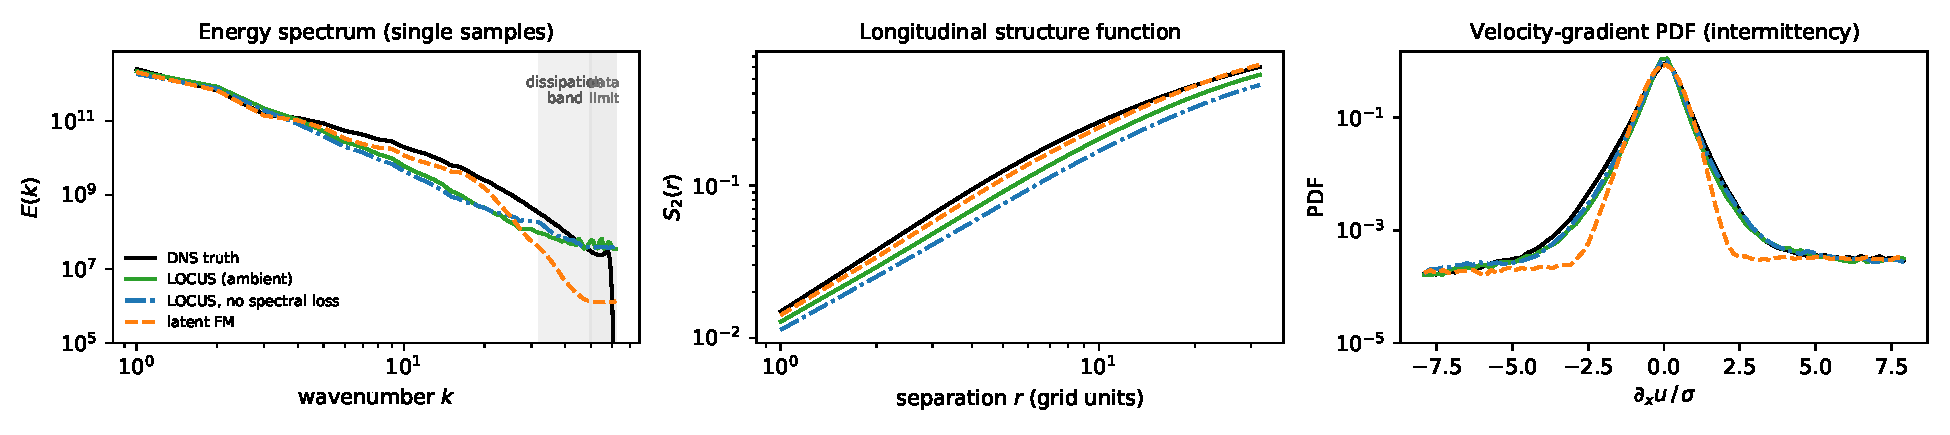
\includegraphics[width=0.92\linewidth]{figures/spectra_stats.pdf}
\end{center}
\caption{\textbf{Turbulence statistics of single posterior samples} on the held-out region (4 snapshots, NFE 4, Hann-windowed; ensemble means are deliberately not shown---averaging destroys small scales by construction). Left: shell-averaged energy spectra. The latent baseline tracks the DNS through the inertial range and then falls away sharply in the dissipation band (shaded), the autoencoder floor; \model{} sits below the DNS through the inertial range and instead flattens into a plateau, which is broadband noise rather than recovered structure. Beyond $k\approx50$ the DNS itself is resolution-limited (light shading). Middle: longitudinal structure functions. Right: velocity-gradient PDFs, where the latent baseline distorts the shoulders while both \model{} variants track the DNS shape.}
\label{fig:spectra}
\end{figure}

\begin{figure}[h]
\begin{center}
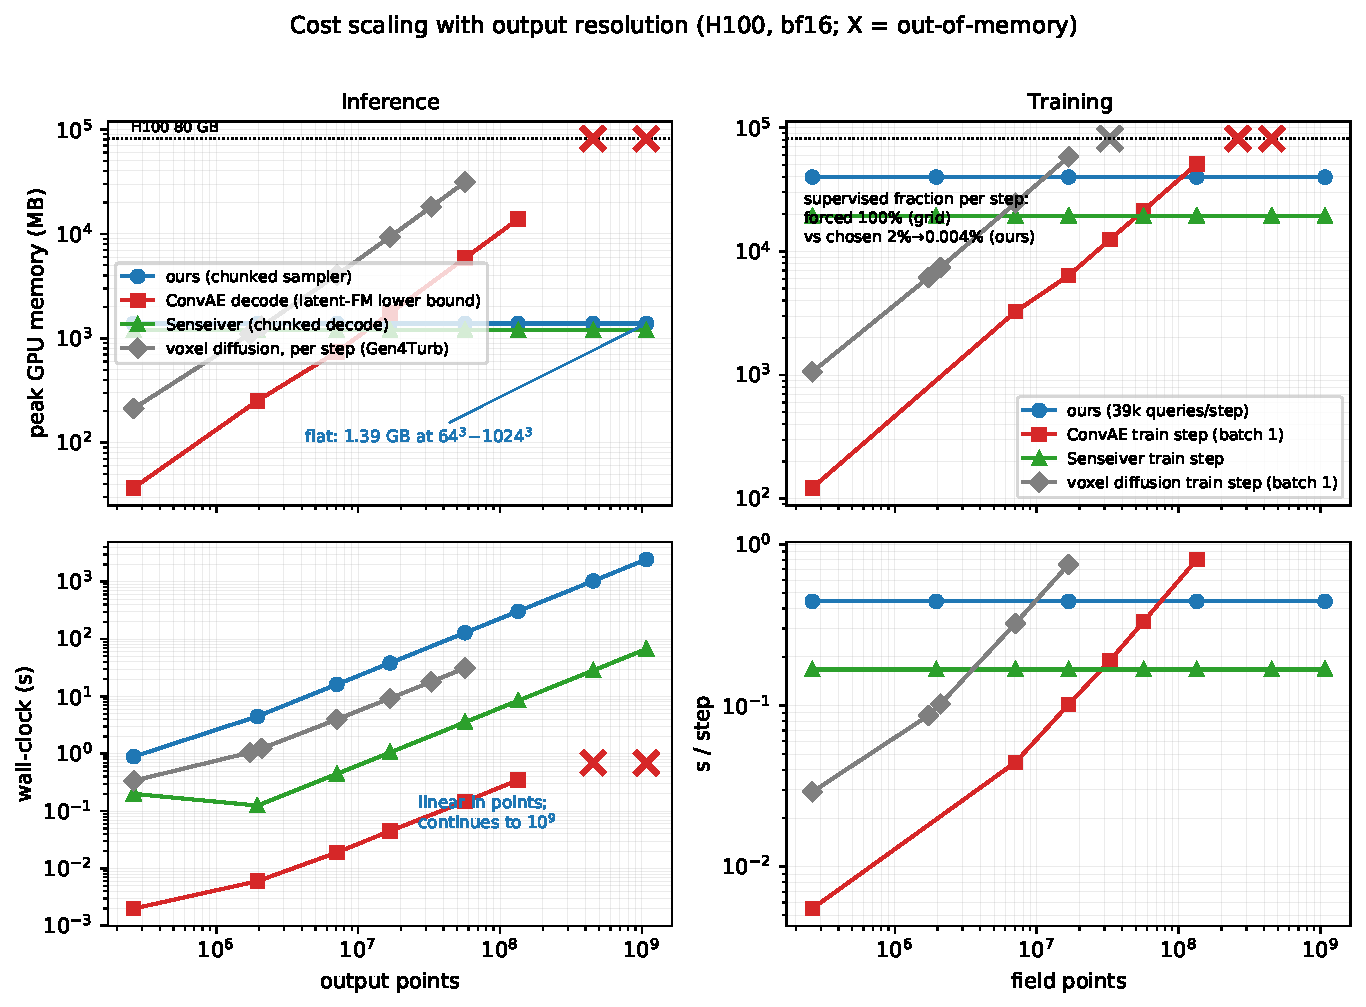
\includegraphics[width=0.9\linewidth]{figures/scaling_cost.pdf}
\end{center}
\caption{Full cost-scaling measurement: peak memory (top) and wall-clock (bottom) for inference and training. The wall-clock panels show the honest converse of the memory result---\model{}'s inference time is linear in the number of evaluation points and is the slowest in absolute terms at large resolution, while its training step time is flat.}
\label{fig:scaling-full}
\end{figure}

\begin{figure}[h]
\begin{center}
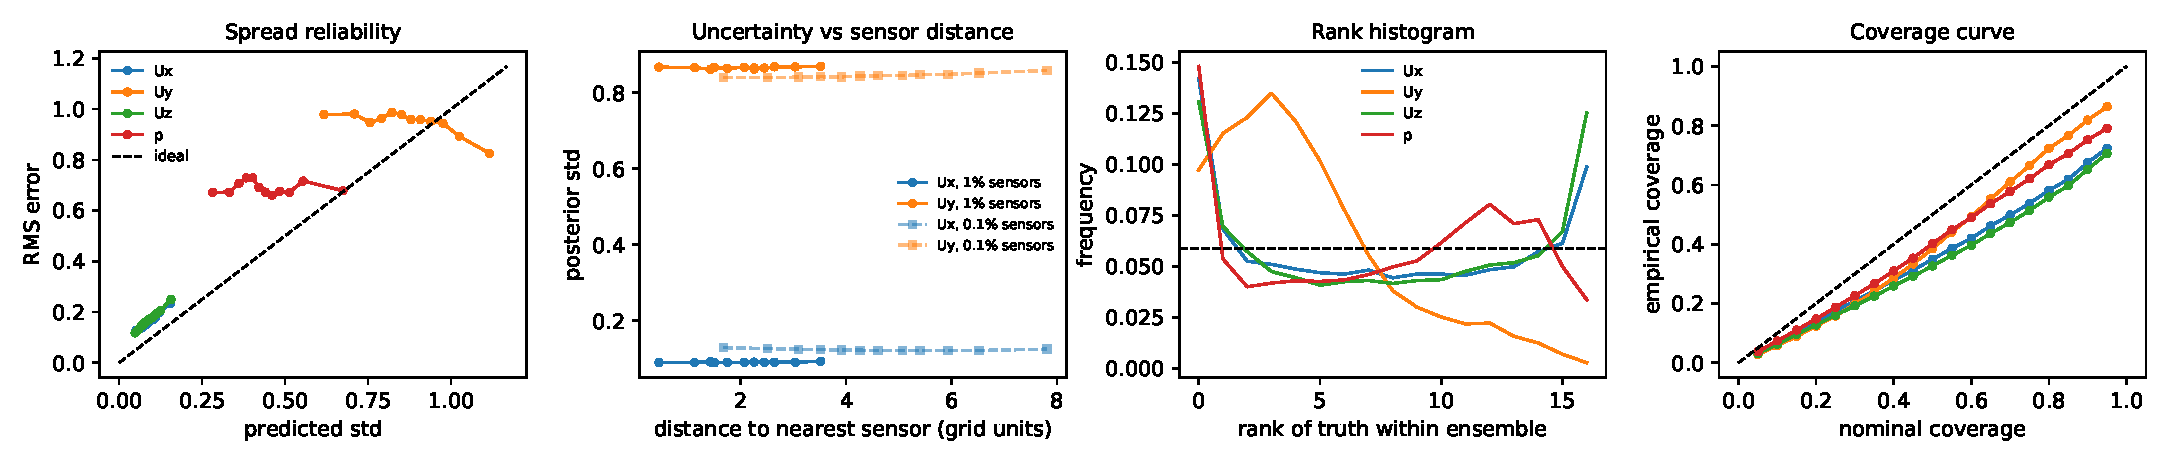
\includegraphics[width=\linewidth]{figures/uncertainty_jhu.pdf}
\end{center}
\caption{Pointwise uncertainty diagnostics on the held-out cube. \emph{Spread reliability}: binned RMS error against predicted standard deviation, ideal on the diagonal; the curves are monotone but above it, the pointwise signature of underdispersion. \emph{Sensor distance}: spread grows with distance to the nearest sensor but saturates against a hard ${\approx}0.09$ floor near the data; expressed against distance, the same profile holds at 1\% and 0.1\% coverage (density-invariant), and NFE rescales it wholesale (${\approx}1.5\times$ from NFE 4 to 16). \emph{Rank histogram}: U-shaped for the observed channels (underdispersed) and sloped for $U_y$ (biased, as expected for a channel no sensor constrains). \emph{Coverage curve}: empirical against nominal central-interval coverage.}
\label{fig:unc-jhu}
\end{figure}

\begin{figure}[h]
\begin{center}
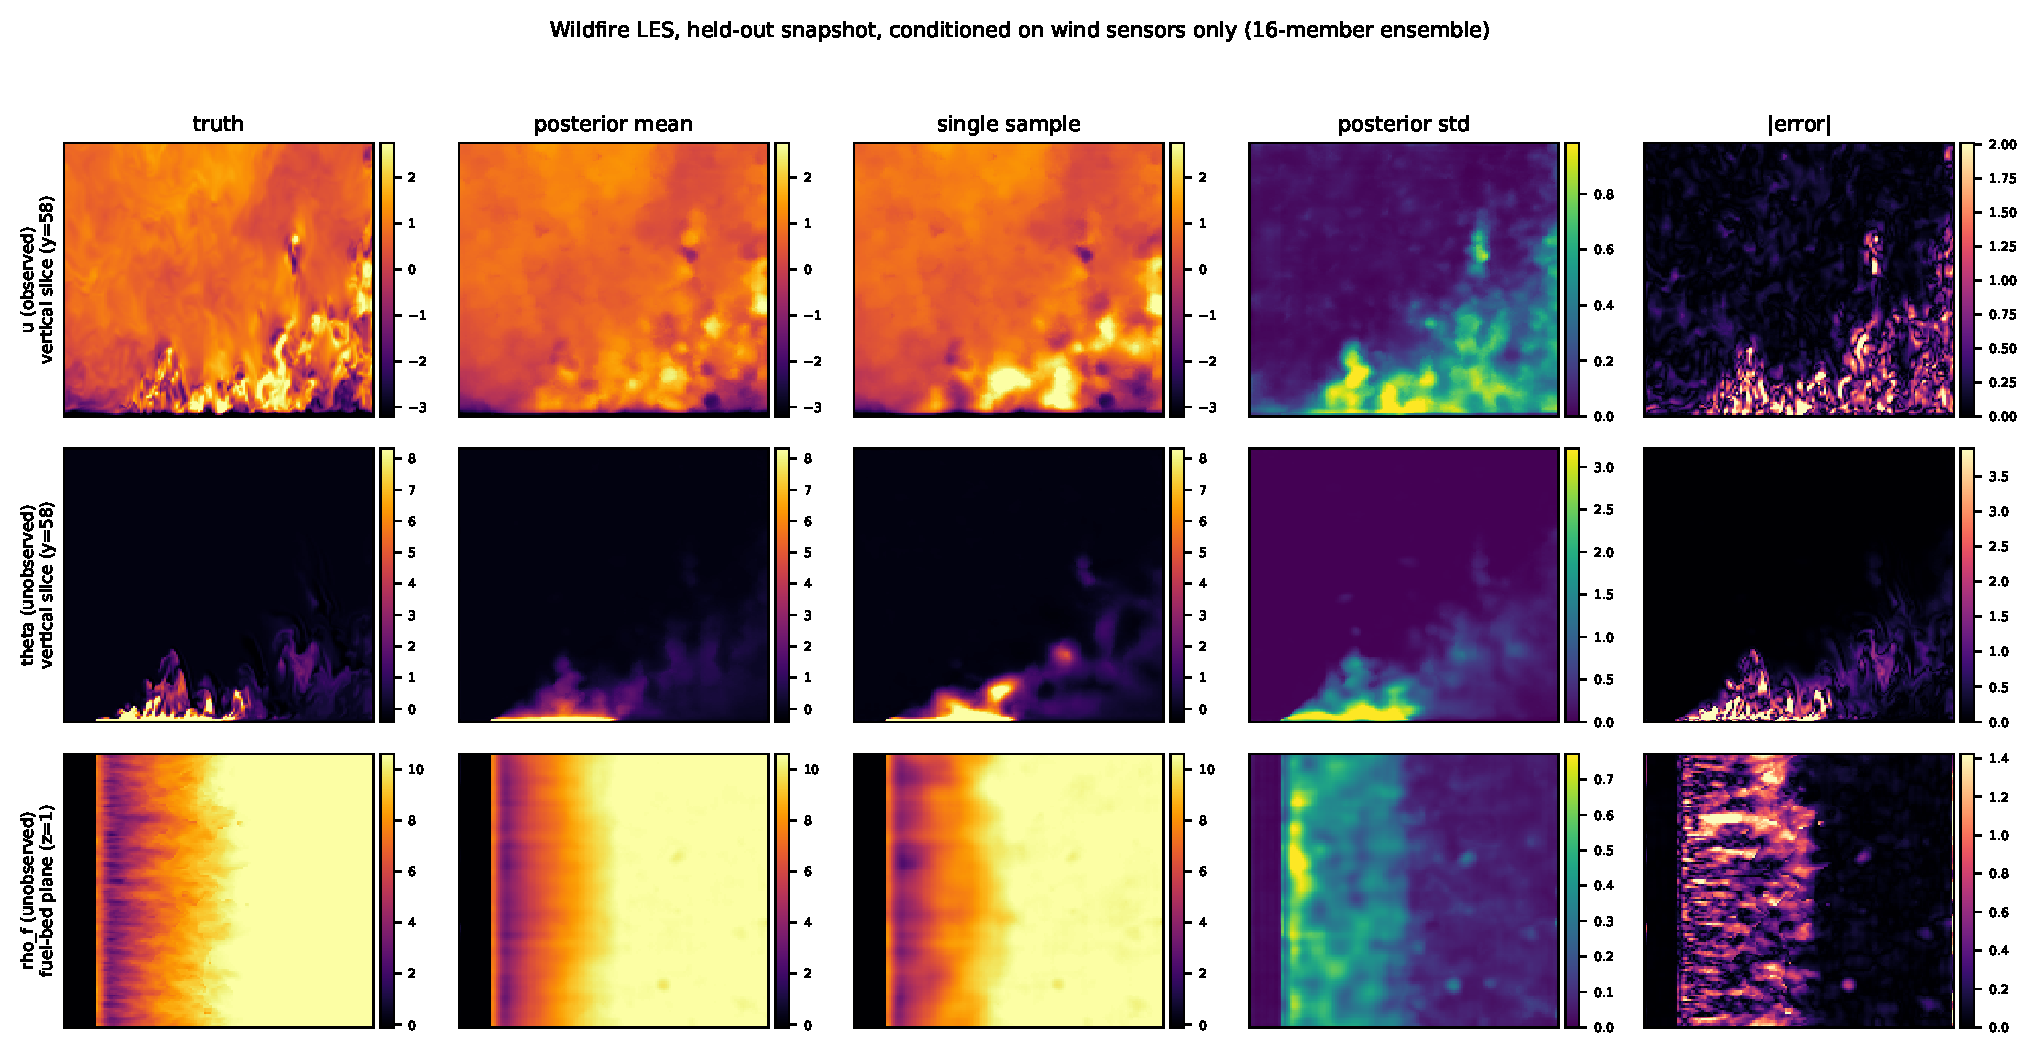
\includegraphics[width=\linewidth]{figures/qual_firebench.pdf}
\end{center}
\caption{Wildfire LES, held-out snapshot, conditioned on wind sensors only. Wind and potential temperature are shown on a vertical slice through the plume; fuel density is shown on the fuel-bed plane, where its structure lives. Potential temperature and fuel density are never observed. From wind alone the model localizes the burn scar and its ragged front, and the predictive standard deviation concentrates on that front---the reconstruction is confident in the burned and unburned interiors and uncertain exactly where the front sits.}
\label{fig:qual-fb}
\end{figure}

\begin{figure}[h]
\begin{center}
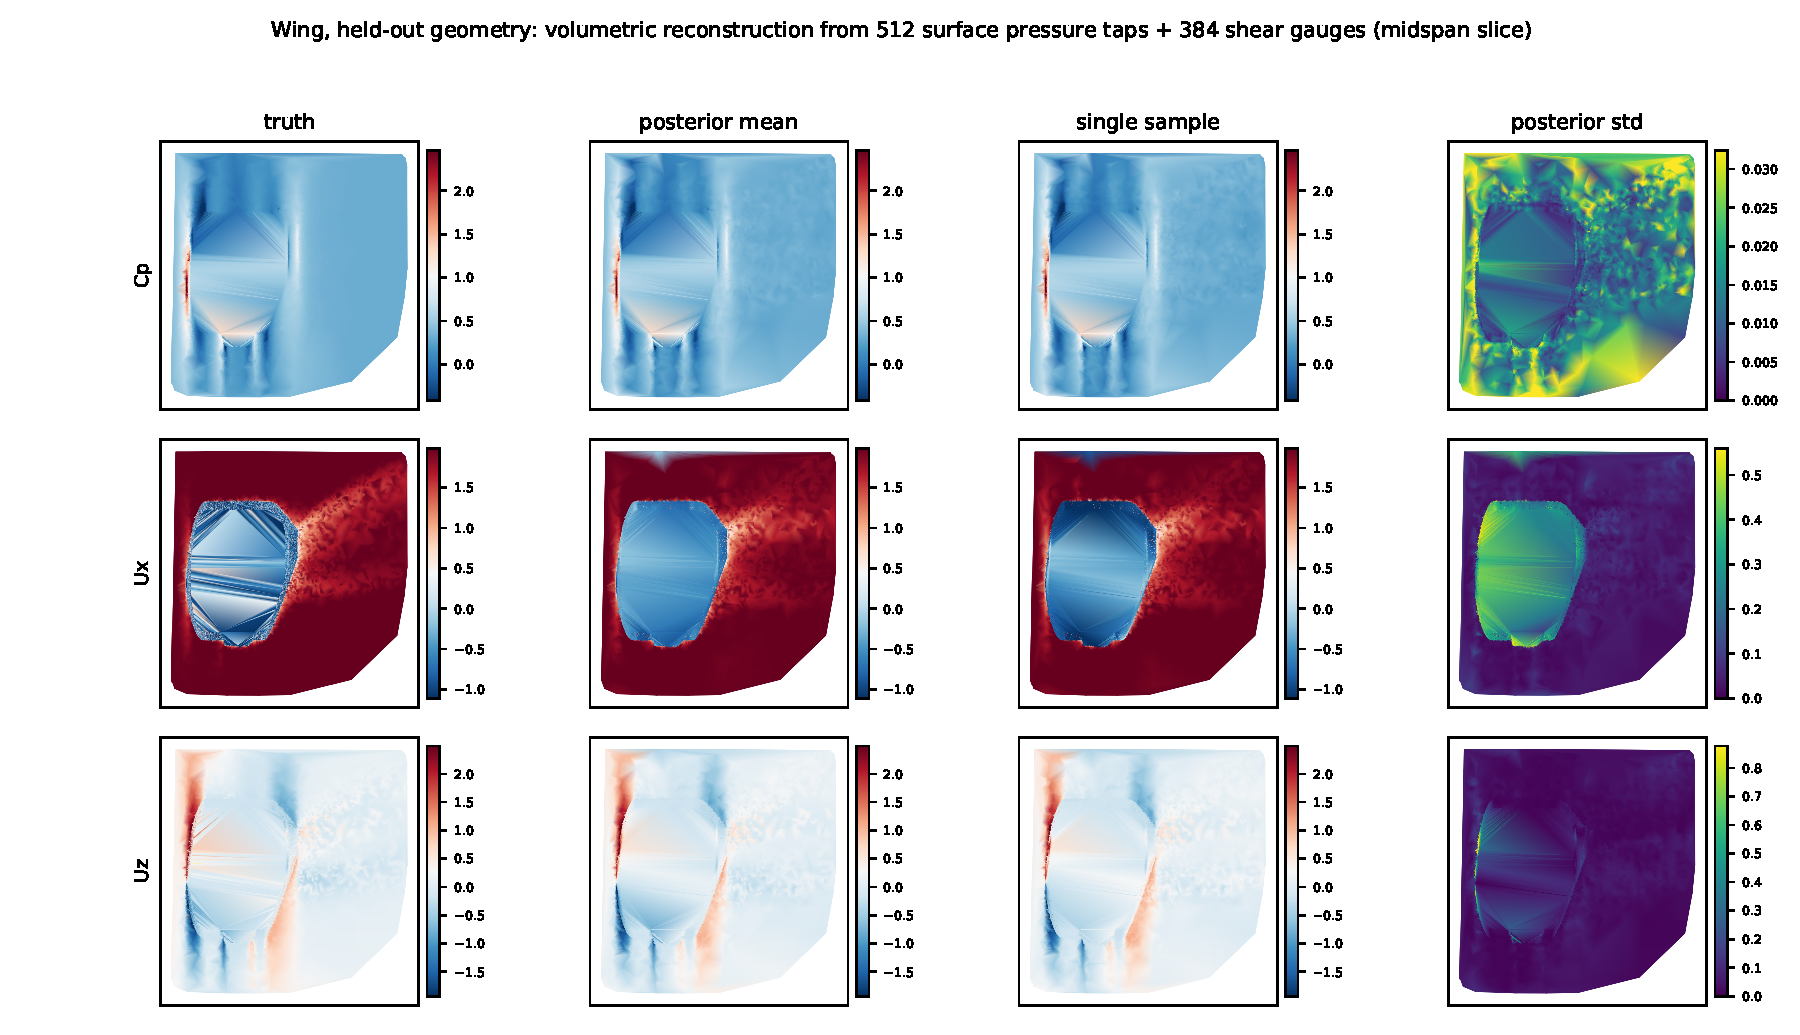
\includegraphics[width=0.92\linewidth]{figures/qual_wing.pdf}
\end{center}
\caption{Wing, held-out geometry, midspan slice: volumetric reconstruction from surface pressure taps and shear gauges alone. The predictive standard deviation is largest in the boundary layer and wake---the regions surface data does not determine---and the standard deviation and error decay together away from the skin (Figure~\ref{fig:unc-wing}).}
\label{fig:qual-wing}
\end{figure}

\begin{figure}[h]
\begin{center}
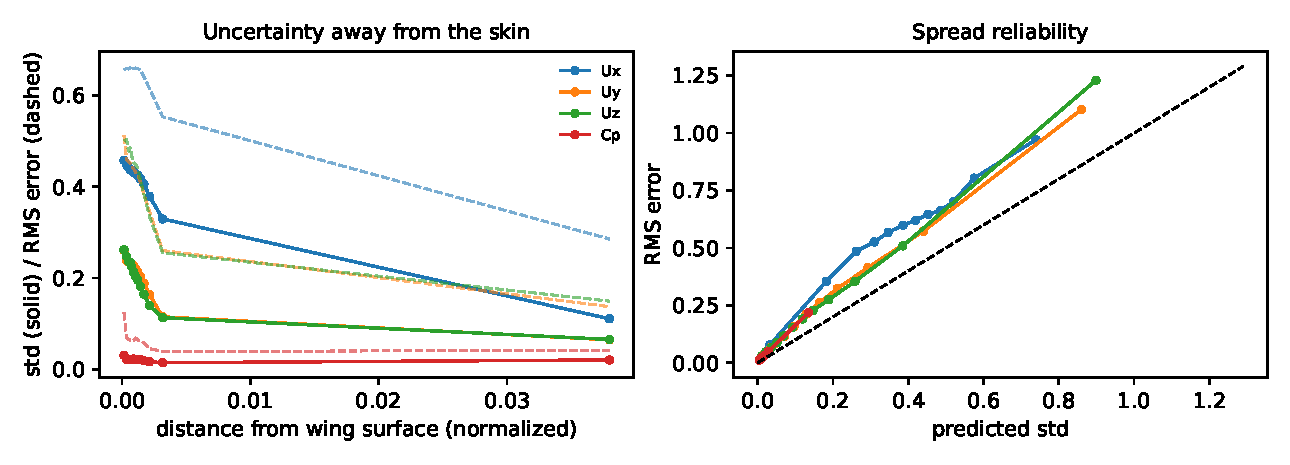
\includegraphics[width=0.75\linewidth]{figures/uncertainty_wing.pdf}
\end{center}
\caption{Wing uncertainty profiles. Left: predictive standard deviation (solid) and RMS error (dashed) against distance from the wing surface; both decay together, so the spread is informative about where the reconstruction is trustworthy. Right: spread reliability, again monotone and above the diagonal. Pointwise correlation between standard deviation and error is 0.77 on this case.}
\label{fig:unc-wing}
\end{figure}

\paragraph{Pending additions.} \todo{Ordered per HANDOFF 2026-08-30: (P1) wing/FireBench baseline tables and figures per the gap analysis (wing: Senseiver/latent FM/CoNFiLD/gappy POD/SiT-point rows $+$ ``n/a without resampling'' rows; pathway ablation; tap sweep; galleries); (P3) recalibration TEST-split numbers, both estimators, ours $+$ latent FM; then: S3GM canonical row and improvement-arm rows; paired per-snapshot CIs vs.\ SiT-point and latent FM; training-seed replicates; density-sweep/Pareto figure; member-level spectra for SiT-point and repaired latent FM; discretization-transfer experiment ($500^3$ cutout $+$ irregular/coarsened point sets); architectural ablations (GP source vs.\ i.i.d., global/local pathway, importance bias); further OOD operators on wildfire; rank-histogram figure.}

\end{document}
